% -*- root: ../main.tex -*-
%!TEX root = ../main.tex
% this file is called up by main.tex
% content in this file will be fed into the main document
% vim:textwidth=80 fo=cqt

\clearpage
\chapter{Implementing a New Electrolyte Model for the \glsfmtshort{spm}}\label{ch:newelectrolytemodel}
\startcontents[chapters]
\printcontents[chapters]{}{1}{\setcounter{tocdepth}{1}}

% change according to folder and file names
\graphicspath{{6/figures/}}

% A suitable  family of models from  the broad category of  reduced-order models
% is  identified  as  a  promising  candidate  for  implementation  in  controls
% applications.
\bigskip

% % -*- root: ../main.tex -*-
%!TEX root = ../main.tex
% this file is called up by main.tex
% content in this file will be fed into the main document
% vim:textwidth=80 fo=cqt


\capolettera{T}{his} chapter presents the  author's attempts towards arriving at
an  accurate description  of the  spatio-temporal evolution  of the  electrolyte
concentration. The  performance of the quadratic  approximation model introduced
in \cref{ch:spmanalysis} is analysed through the novel application of a symbolic
regression framework that  helped to expose the issue of  equation deficiency in
the underlying \gls{dfn}  model for the purpose of electrolyte  modelling with a
pre-assumed model  structure. Although this  framework did not  ultimately yield
the desired outcomes, it did nevertheless facilitate a comprehensive analysis of
the strengths and weaknesses of the  quadratic approximation model which has not
been performed in existing literature. Next, the author's unique contribution to
the art  of single  particle modelling  \viz{} a  novel time-evolution  model of
electrolyte  concentrations through  the technique  of system  identification is
presented. The  results of  the new  approach is  compared against  the baseline
quadratic approximation model. Finally, the new model equations are incorporated
into  an electrolyte-enhanced  \gls{spm} and  the performance  of the  composite
model is compared against the conventional \gls{spm},



% \section{Performance Analysis: Quadratic Approximation Model}\label{sec:symbolicregression}
% % -*- root: ../main.tex -*-
%!TEX root = ../main.tex
% this file is called up by main.tex
% content in this file will be fed into the main document
% vim:textwidth=80 fo=cqt


In the  author's analysis of the  quadratic approximation model, the  origin and
nature of  its sub-optimal  performance can  be explained  as per  the following
rationale. The quadratic  approximation model uses a  bottom-up approach wherein
the final  simplified model structure  is pre-assumed  and then the  physics are
made  to  fit  within  this  framework. Given  that  the  top-down  approach  to
electrolyte  modelling, \ie{}  accounting for  all physical  phenomena and  then
simplifying  them yields  mathematically intractable  and overly  complex models
(see~\cref{sec:electrolyteinclusion} for  a detailed discussion),  this approach
seems to be a pragmatic alternative  to enhancing the \gls{spm} with electrolyte
dynamics. However, a detailed look at  this model from an alternate viewpoint is
necessary for further analysis.


\subsection{Symbolic regression using \glsfmtlong{mggp}}

The  question boils  down to  whether a  quadratic approximation  is indeed  the
\emph{best}  model structure  that  can  be assumed  a  priori  for the  spatial
profile  of  ionic  concentration  in  the  electrolyte.  This  author  embarked
on  a journey  to  find  suitable alternate  model  structures,  \ie{} a  single
family of  curves that can  capture both  the transient and  \gls{qss} behaviour
exhibited by  the ionic  concentration. The open-source  \textsc{MATLAB} toolbox
GPTIPS2~\cite{Searson2015}  uses the  state-of-the-art  \gls{mggp} approach  for
symbolic data  mining and is ideally  suited for such symbolic  regression tasks
(fitting a  mathematical equation structure,  and not merely  obtaining best-fit
coefficients to a  pre-assumed curve as in classical numerical  regression, to a
given data).

In employing the \gls{mggp} approach, it  is important to recognize that the key
criteria that restricts
\begin{enumerate*}[label=\emph{\alph*})]
    \item the choice of  gene-sequence depth, as well as
    \item the choice in number of parent mutations,
\end{enumerate*}
is  the   total  number  of   unknown  symbolic  coefficients  required   to  be
solved  in the  assumed  model  structure. There  are  a  total of  \emph{seven}
linear   equations  available   from  the   physics  of   the  \gls{dfn}   model
(see~\crefrange{eq:cecontinuitynegsep}{eq:Qepbyintegration}). Hence, in order to
guarantee  a solution  the  assumed  family of  curves  cannot  consist of  more
than  seven coefficients.  Furthermore, for  a  unique solution,  the number  of
coefficients must be \emph{exactly} seven. Yet another restriction on the choice
of locus of feasible  curves arises due to the fact that  the behaviour of ionic
concentration  in the  negative and  positive electrode  regions are  similar in
complexity\footnote{\label{fn:complexity}The  concept  of complexity  of  curves
used  here is  not  based on  a  precise mathematical  definition  such as  that
employed by Neumann-Coto and Arenas~\cite{Neumann-Coto2017}, but is loosely used
to simply  convey an empirical sense  of their curvature. However,  the analysis
here applies  to the more  rigorous definition as well.},  and hence need  to be
mathematically described by an identical family of curves.

Upon a close inspection of the  spatial concentration profile from the \gls{p2d}
simulation  results shown  in~\cref{fig:spatialionicconc1C}, it  is evident  the
electrolyte approximation  functions within the  electrode regions is  of higher
complexity\textsuperscript{\ref{fn:complexity}} than  the approximation function
suitable  for  use  in  the  separator  region. Based  on  the  results  of  the
quadratic  model, it  is  clear  that at  least  two  coefficients are  required
within the  electrode regions \ie{}  $n_{\text{c,elec}} \ge 2$. There  exists an
inhibiting  factor that  prevents  the  use of  a  lower  order function  within
the  separator. As  per  the  simulation results  of  the  \gls{p2d} model,  the
time-domain  change  of number  of  moles  per  square  meter in  the  separator
is  non-zero.  Since  the  time-derivate   of  a  linear  approximation  applied
to~\cref{eq:sepliionmolesquadratic}  is  zero,  this straight-line  equation  is
immediately ruled out. Among the  non-polynomial mathematical curves tried (such
as trigonometric, hyperbolic, power series  among others), none could obtain the
relatively simple shape of the separator function without being forced to reduce
the  contribution from  one  of  the coefficients  to  below machine  precision.
This necessitates  the retention  of the  quadratic approximation  function used
thus  far  (with  no  missing  terms) \ie{}  $n_\text{c,sep}  =  3$.  Thus,  the
overall number  of coefficients in the  best possible approximation shall  be $2
n_\text{c,elec} + n_\text{c,sep} =  2\cdot2 + 3 = 7$, which  is the total number
of electrolyte-specific physical constraints available from the \gls{dfn} model.
Hence it  can be concluded  that the  quadratic approximation model  does indeed
make the \emph{best}  use of all of the available  physical equations. The final
question remains to  answer is, with these coefficient  limitations, whether the
quadratic  equation structure  indeed  the optimal  one.  This was  investigated
through the \gls{mggp} approach described next.

The GPTIPS2  toolbox uses a variety  of heuristic algorithms from  the theory of
\gls{mggp}  to hypothesise  a suitable  equation structure  for the  data to  be
fitted.  The dataset  consisted of  the  simulation results  from the  \gls{p2d}
model,  in particular  the  values  of electrolyte  concentration  at the  three
different cell  regions captured  at various snapshots  of time.  Both transient
and  \gls{qss} data  were  fed into  this  symbolic data  mining  process and  a
single all-encompassing  family of curves  capable of capturing  the electrolyte
concentration behaviour was  sought for. However, the constraints  in the number
of coefficients that  can be employed results  in a restriction of  the depth of
gene  mutations as  well  as the  number of  parent/seed  populations. The  best
equation set  (without strictly  enforcing the aforementioned  hard constraints,
yet  minimizing  the  distance  to  the constraint  vector)  that  the  symbolic
regression approach yielded was
\begin{alignat}{2}
    c_\ensub(z,t) & = a_2(t) \cosh z^2 + a_1(t) \sinh z + a_0(t) \qquad &  & 0 \le z \le l_\text{n} \label{eq:cnstrviolneg} \\
    c_\essub(z,t) & = a_5(t) z^2 + a_4(t) z + a_3(t) \qquad             &  & 0 \le z \le l_\text{s}                         \\
    c_\epsub(z,t) & = a_8(t) \cosh z^2 + a_7(t) \sinh z + a_6(t) \qquad &  & 0 \le z \le l_\text{p}\label{eq:cnstrviolpos}
\end{alignat}

Although~\crefrange{eq:cnstrviolneg}{eq:cnstrviolpos}  fit   the  transient  and
\gls{qss}  profiles  well,  they  violate   the  constraint  on  the  number  of
coefficients  available resulting  in  an underdetermined  system of  equations.
Both  the least-squares  and  least-norm  solution of  this  system were  tried.
However, the  results were inferior to  that produced by the  baseline quadratic
approximation method.

Next, an  attempt was made to  obtain different mathematical structures  for the
transient phase  and \gls{qss}  phase both  of which  respect the  constraint on
number  of  coefficients  allowed.  The symbolic  regression  outputs  for  this
approach are shown in~\cref{tbl:symbreg}.
% -*- root: ../main.tex -*-
%!TEX root = ../main.tex
% this file is called up by main.tex
% content in this file will be fed into the main document
% vim:nospell textwidth=180 foldlevelstart=3 foldlevel=3 conceallevel=0

\begin{table}[!htb]
    \centering
    \caption[Transient \& \glsfmtshort{qss} expressions for electrolyte
    concentration obtained by \glsfmtshort{mggp}]{Best fit expressions for the
        transient and \glsfmtlong{qss} approximaton functions for the
    electrolyte functions obtained by the \gls{mggp} approach}
    \label{tbl:symbreg}
    \begingroup
    \addtolength{\jot}{0.25em}
    \begin{tabular}{@{} c c r @{}}
        \toprule
        \multicolumn{1}{l}{Transient Function} & \multicolumn{1}{c}{\glsfmtlong{qss} Function} & \multicolumn{1}{c}{Region} \\
        \midrule
        $\begin{aligned}
            c_{\text{e,n}_\text{trans}} &= a_1 z^6 \ln z^6 + a_0 \\
            c_{\text{e,s}_\text{trans}} &= a_4 z^2 + a_3 z + a_2 \\
            c_{\text{e,p}_\text{trans}} &= a_6 z^6 \ln z^6 + a_5 \\
        \end{aligned}$ &
        $\begin{aligned}
            c_{\text{e,n}_\text{QSS}} &= a_1 \sinh z^2 + a_0 \\
            c_{\text{e,s}_\text{QSS}} &= a_4 z^2 + a_3 z + a_2 \\
            c_{\text{e,p}_\text{QSS}} &= a_6 \sinh z^2 + a_5
        \end{aligned}$ &
        $\begin{aligned}
            &0 \le z \le l_\text{n} \\
            &0 \le z \le l_\text{s} \\
            &0 \le z \le l_\text{p}
        \end{aligned}$
        \\
        \bottomrule
    \end{tabular}
    \endgroup
\end{table}



Although  the equations  from~\cref{tbl:symbreg}  produced  a markedly  improved
response during the transient phase,  the performance during the \gls{qss} phase
was merely at par to the baseline quadratic approximation model. This raised the
prospect of  employing a  blended approach, wherein  a model  changeover between
the  transient  and \gls{qss}  was  contemplated.  However,  since there  is  no
precise definition  of what constitutes  the transient phase of  the electrolyte
concentration response, this  approach required some ad-hoc  timing criteria for
correctly  transitioning  between  the  two \gls{mggp}  equation  sets.  Further
complications arise  during dynamic input conditions,  wherein the concentration
profiles are mostly in a state of  flux and could linger for longer durations at
the contiguous  boundary between  transient-like and  \gls{qss}-like behaviours.
In  the  interest  of  reproducibility  across  different  cell-chemistries  and
corresponding parameter sets, the proposed blended model transition approach was
not further pursued.

Overall,  the  long  and  arduous  process of  symbolic  regression  was  not  a
definitive  success in  this  case  mainly due  to  the  limitation of  equation
deficiency of physical constraints. Perhaps  if yet another physics-based model,
\ie{} an  alternative to the  widely prevalent \gls{dfn}  model, can be  used as
the  baseline,  a  few  more  physical governing  equations  could  possibly  be
made  available. This  can perhaps  result in  a less  restrictive gene-set  for
coefficient  determination  and  consequently  pave the  way  for  a  successful
implementation  through  this  hitherto  unexplored  route  of  \gls{mggp}-based
equation synthesis.

In conclusion,  the quadratic model for  electrolyte concentration approximation
makes the  best use of the  available physical equations. Given  the constraints
with  respect to  physical equations  discussed here,  it is  also deemed  to be
the  optimum  family  of  a  priori  chosen  curves  capable  of  modelling  the
\emph{spatial}  profile of  ionic concentration.  Notwithstanding these  merits,
the  \emph{temporal}  performance of  the  quadratic  approximation approach  is
sub-optimal as seen in~\cref{fig:temporalcequadratic}. The author of this thesis
addresses this specific issue with a completely different approach that shall be
discussed next in~\cref{sec:newelectrolytemodel}.



% \section{A New Electrolyte Model through System Identification}\label{sec:newelectrolytemodel}
% % -*- root: ../main.tex -*-
%!TEX root = ../main.tex
% this file is called up by main.tex
% content in this file will be fed into the main document
% vim:textwidth=80 fo=cqt

Having performed a  comprehensive analysis of the state of  the art in \gls{spm}
modelling, this section presents the  author's unique contribution to the field.
Firstly, the  scope of the  contribution is identified. The  methodology adopted
and corresponding results are presented thereafter.

\subsection{Scope and motivation}\label{subsec:scopenewelectrolyte}

This subsection is intended as a capstone summary helping to briefly recount the
discussion so far  and to provide a  context for the author's work  in the wider
realm  of the  \gls{spm}  modelling art.  In  the same  vein  as the  discussion
in~\cref{sec:electrolyteinclusion}, the scope of the proposed enhancement to the
\gls{spm} concerns entirely  with improving the electrolyte subsystem  as it has
already been established in~\cref{subsec:simresultsbasicspm} that the simplified
representation of  the solid-phase subsystem  through a fourth  order polynomial
approximation method  for diffusion of  \ch{Li^0} in  the solid particle,  is of
sufficiently high accuracy.

Inspecting the  electrolyte domain,  the electrolyte  overpotential contribution
to  terminal  voltage   consists  of  a  diffusion   overpotential  in  addition
to   the  time-dependent   ohmic  losses   that  originates   from  differential
concentration  gradients  that  is   indirectly  dependent  upon  concentration.
Hence,  accurate  determination  of   spatio-temporal  concentration  takes  the
centre  stage.  For   the  computation  of  overpotential   in  the  electrolyte
phase,~\cref{eq:electrolytepdwithce}  proposed  by  Prada~\etal~\cite{Prada2012}
may be used.

There exists a  subtle detail in the  use of~\cref{eq:electrolytepdwithce} which
is discussed here upfront before proceeding  ahead to the refined context of the
author's  work.  The  intrinsic  conductivity  of  electrolyte,  $\kappa$  is  a
function of  the ionic concentration  (refer~\cref{subsec:basicspmsimsetup}). If
the ionic  concentration at  the corresponding current  collectors are  used for
$\kappa_\text{neg}$  and  $\kappa_\text{pos}$, this  would  lead  to a  lopsided
computation of the overpotential in electrolyte. Furthermore, under this scheme,
the computation of electrolyte conductivity shall be rendered ambiguous since it
is unclear which  separator interface shall be chosen for  the separator's ionic
concentration. Although this  has not been discussed clearly  in literature, the
author  of this  thesis chose  to use  the mean  concentration within  each cell
region, defined as
\begin{equation}
    \mean{c}_{\text{e},j}(t) = \frac{1}{l_j}\int_0^{l_j} c_{\text{e}_j}(z,t)\, dz = \frac{Q_{\text{e,}j}(t)}{\varepsilon_j l_j}
\end{equation}
although other measures  of central tendency might be equally  valid. Hence, the
results of this section have the associated variability in them depending on how
the electrolyte concentration computations are  used in evaluating the intrinsic
conductivity of electrolyte.

As  the  ionic  concentration  has  both  a  direct  and  indirect  contribution
in~\cref{eq:electrolytepdwithce}, its spatio-temporal  computation is a critical
aspect. As discussed  in~\cref{sec:quadraticapprox}, the quadratic approximation
is a widely used spatio-temporal model for electrolyte concentration which makes
the best  use of available physical  constraints. As established in  the results
of~\cref{subsec:quadraticsimresultsanalysis}, while  the spatial  performance of
the quadratic approximation approach is acceptable, its time-domain performance,
particularly at the crucial current collector locations is mediocre at best.

Thus,   the  \emph{scope}   of  the   author's  work   is  to   obtain  suitable
alternate   expressions   for   improving  the   computation   of   \textbf{time
evolution}  of  the electrolyte  concentration  whilst  retaining the  quadratic
approximation   approach   for  describing   its   spatial   profile.  Such   an
approach  is motivated  by  the  keen observation  that  the baseline  quadratic
approximation  model  has  a  natural  `pause'  in  its  model  description.  To
clarify,~\crefrange{eq:cecontinuitynegsep}{eq:Qepbyintegration}  form a  tightly
coupled set of  seven linear equations in seven unknowns.  The time evolution of
$Q_{\text{e,}j}$  are described  through  a system  of  first order  \glspl{ode}
given by~\crefrange{eq:negliionmolesquadratic}{eq:posliionmolesquadratic}.  In a
practical  implementation,  these  \glspl{ode}  are solved  independently  in  a
decoupled  manner,\ie{}  by using  the  coefficients  obtained from  the  linear
system of~\crefrange{eq:cecontinuitynegsep}{eq:Qepbyintegration} in the previous
time-step. The  author's hypothesis is that  by taking advantage of  the natural
break  in the  operational  sequence which  involves  two separate  computations
between  two independent  subsystems (for  all practical  purposes), it  must be
possible  to  replace  the  underperforming time-evolution  equations  from  the
baseline quadratic approximation with a superior alternate model.

\subsection{Background and Rationale}\label{subsec:sysidbackground}
% might have to change section title if TF-based identification becomes a full-fledged subsection

% This section presents the methodology adopted in obtaining an improved model for
% the rate of evolution  of overall moles per unit area of  \ch{Li^+} ions in each
% of the three regions of the cell.

This  section presents  the  background and  thought  process in  systematically
arriving  at  the  choice of  the  methodology  that  was  adopted for  the  new
time-evolution model of the electrolyte concentration.

Based  upon the  experience  gained  in dealing  with  the literature  presented
in~\cref{sec:electrolyteinclusion}, it is  the author's view that,  owing to the
complex behaviour of electrolyte, a  naive top-down approach \ie{} including all
the physics upfront  followed by a systematic simplification, might  result in a
model that is  mathematically intractable for adoption in  an embedded \gls{bms}
environment.  The baseline  quadratic  approximation method  has  proven that  a
bottom-up  approach, \ie{}  pre-assuming a  simplified structure  for the  final
model  and adapting  its coefficients  to physical  constraints yields  a viable
candidate for inclusion in the conventional \gls{spm}.

Upon  a   closer  examination   of  the  rubrics   of  the   baseline  quadratic
approximation  model, it  comes  to  light that  the  natural `pause'  discussed
towards  the  end  of~\cref{subsec:scopenewelectrolyte}  permeates  to  a  level
more  than  merely  having  to  operate  sequentially  on  two  pseudo-decoupled
subsystems  --- it  goes to  the extent  of rendering  the operating  philosophy
of  fitting  physical  equations  semi-void.   To  clarify  this  statement  and
to  substantiate   the  claim,  while  there   is  no  doubt  that   the  linear
algebraic   equations  of~\crefrange{eq:cecontinuitynegsep}{eq:Qepbyintegration}
do    incorporate    physical    principles   from    the    \gls{dfn}    model,
the     same     does     not      hold     true     for     the     \glspl{ode}
of~\crefrange{eq:negliionmolesquadratic}{eq:posliionmolesquadratic}.   In  fact,
all   the   boundary   conditions   from   the   \gls{dfn}   model   have   been
exhausted   by  this   stage  (refer~\cref{subsec:quadraticsimresultsanalysis}).
Although~\crefrange{eq:negliionmolesgen}{eq:posliionmolesgen}     are    derived
from     the      \gls{dfn}     model,      the     coefficients      of     the
diffusivities   in    the   \gls{rhs}   of    the   next   set    of   equations
\ie{}~\crefrange{eq:negliionmolesquadratic}{eq:posliionmolesquadratic},   merely
involve  substitutions  of the  spatial  derivatives  of the  assumed  quadratic
expression.

Herein lies the weakness of the  baseline quadratic approach. Unlike the spatial
algebraic equations, which are tightly bound by the continuity and flux boundary
conditions at the  separator interfaces, there is no equality  constraint on the
spatial  derivative, which  is free  to grow  or shrink  without any  explicitly
imposed  bounds.  The  onus  of  being accurate  is  therefore  on  the  spatial
derivative evaluation which in-turn depends  on the correctness of the quadratic
functions~(\crefrange{eq:cenquadreduced}{eq:cepquadreduced})  themselves. It  is
not feasible to quantify the magnitude of error introduced in the time-evolution
of concentration  given a small-signal  perturbation in the coefficients  of the
quadratic spatial  computation,\ie{} the implicit  coupling between them  is not
transparent. Since the quadratic approximation itself is not perfect, \ie{} does
not capture the  spatial gradient \emph{exactly} as the \gls{p2d}  model as seen
in~\cref{fig:spatialionicconc1C}, the internal coupling of coefficients leads to
errors in time-evolution computation.

The author's  approach is to  therefore break this detrimental  coupling between
spatial  derivative of  concentration  and its  temporal evolution  counterpart.
Inspired by the fact that the  quadratic approximation model had almost achieved
the desired goals with
\begin{enumerate}[label=\emph{\alph*})]
    \item a bottoms-up approach, \ie{} assuming some model structure apriori, and
    \item not bound by any physical considerations due to the exhaustion of governing equations
\end{enumerate}
have led  the author  to broach  a modelling concept  that exhibit  these common
traits,  yet  of  a  completely  different nature  and  hitherto  unexplored  in
physics-based  battery  modelling  in   general  and  electrolyte  modelling  in
particular --- \emph{black-box system identification}.

\subsection{Brief Introduction to System Identification}\label{subsec:introsysid}

An in-depth  coverage of the topic  of system identification is  well beyond the
scope of  this thesis.  However, keeping  in mind the  interests of  the battery
modelling community  who might not be  familiar with this subject  area, a brief
overview of the core ideas that  are essential for tackling the specific problem
at hand, is presented. For readers  further interested in this topic, the author
suggests the textbook by  Ljung~\cite{Ljung1999} for a comprehensive theoretical
treatment of the foundation topics in system identification.

System identification aims  to provide a mathematical model  of the input-output
mapping  of  a system\footnote{The  precise  definition  of what  constitutes  a
`system' is detailed  in Ljung's textbook. However, for  all practical purposes,
in this  thesis the word `system'  stands for any unknown  entity whose terminal
behavioural model  is being  sought for ---  primarily from  input-output data.}
under consideration. The three categories of system identification are:


\begin{enumdescriptnum}[leftmargin=!,itemsep=1ex,labelwidth=\widthof{$\symbf{\text{brugg}_j}\ \scriptstyle (\times 3)$abc}
    ,partopsep=0pt
    ,topsep=0pt
    ]

\item[White box] wherein underlying physical equations are completely known. The
numerical value  of coefficients of  governing equations are to  be parametrised
from input-output data.

\item[Black box]  wherein no  governing equations are  available for  the system
under  consideration. The  model formulation  is facilitated  by a  rich set  of
system theory  which proceeds by exciting  the system with input  waveforms with
certain desirable  properties and correlating characteristics  from the response
in order  to draw  conclusions about viable  mathematical structures  capable of
emulating  the  terminal  behaviour  of the  system  under  generalised  inputs.
Black  box system  identification was  employed for  the specific  problem under
consideration and hence all future descriptions will pertain to this class.

\item[Grey box] is a hybrid of the  two approaches wherein a part of the model's
governing  physics is  known a  priori, \eg{}  the structure  of a  well-defined
subsystem  that is  part  of a  large,  complex  system may  be  known ahead  of
time,  where the  task  is  to characterise  the  full  system. Grey-box  system
identification tasks can  often be reduced to a single  sub-problem of black-box
system  identification  by  removal  of  the known  physics  and  tackling  them
separately.

\end{enumdescriptnum}

\subsection{Overview of black-box system identification}\label{subsec:introblackboxsysid}
Black-box system identification techniques can be broadly classified into ---
\begin{enumerate*}[label=\emph{\alph*})]
     \item non-parametric methods, and
     \item parametric methods.
 \end{enumerate*}

Non-parametric methods do not seek  a pre-assumed mathematical structure for the
system. They  aim to  directly estimate  the very  kernel of  what characterises
every system \viz{}  the Markov parameters in the time-domain  and the \gls{frf}
in the frequency domain, thereby requiring \emph{infinite} number of data points
for  their representation.  Major non-parametric  system identification  methods
include:
\begin{itemize}[topsep=0pt]
    \item Identification in time domain
        \begin{itemize}

            \item Direct  estimation of the system's  Markov parameters through
                statistical correlation of its response to an unit-pulse input

        \end{itemize}
    \item Identification in frequency domain,  \ie{} of the \gls{frf}
        \begin{enumerate}

            \item   Direct   estimation    through   input-output   statistical
                cross-correlation

            \item  \gls{etfe} using \glspl{dft} of input and output sequences

            \item  Smoothed periodogram estimates using Welch's method

            \item  Blackman-Tukey  estimation   method  using  standard  filter
                windows  in digital  signal processing  (such as  Hamming, Hanning,
                Bartlett, Boxcar etc.)

        \end{enumerate}
\end{itemize}

Parametric  methods  aim  to  fit  specific input-output  data  to  some  family
of  well-known  mathematical  constructs  that  generalise  well  to  a  variety
of  inputs.  It  is  important  to recognise  that,  in  contrast  to  white-box
system identification, the salient coefficients/properties of these mathematical
structures do  not, in any way  correspond to physical properties  of the system
under consideration. Major parametric system identification methods are:
\begin{itemize}
    \item Transfer-function based frequency domain model structures
        \begin{enumerate}
            \item \gls{oe} model
            \item \gls{arx} model
            \item \gls{armax} model
            \item Box-Jenkins (BJ) model
        \end{enumerate}
    \item State-space time-domain model structures
        \begin{enumerate}
            \item Ho-Kalman realisation
            \item \gls{era} realisation
            \item Deterministic and stochastic \emph{subspace} structures
        \end{enumerate}
\end{itemize}

Among  these  system  identification  methods, the  non-parametric  methods  are
immediately  ruled  out   for  applying  to  the  task  at   hand.  As  outlined
in~\cref{subsec:sysidbackground},  the author  is  inspired by  the trait  of
having  a  pre-assumed  model  structure that  brought  the  baseline  quadratic
approximation closer to a successful  realisation. The non-parametric methods do
not conform to this philosophy.  Furthermore, the requirement of infinite number
of data  samples in order to  fully quantify the system  dampens its feasibility
for implementation  in resource constrained  environments. The author is  of the
opinion that resorting  to truncation of the characteristic  sequence shall only
yield a sub-optimal solution.

While  parametric state-space  identification is  a feasible  alternative, these
methodologies  are   tedious  and   error-prone.  For  instance,   applying  the
Ho-Kalman  algorithm requires  construction  of  Block-Hankel matrices  followed
by  a  \gls{svd} operation.  The  \gls{era}  brings  with  an identical  set  of
operations  of  the  Ho-Kalman  procedure, except  that  certain  random  blocks
in  the  Hankel   matrices  are  chosen  at  random  for   deletion  for  better
estimates  in  low \gls{snr}  environments  and  for capturing  slowly  decaying
phenomena  with long  time constants.  The subspace  methods are  mathematically
involved,  requiring  a  profound  understanding of  projections  to  orthogonal
subspaces  from linear  algebra.  The system  under  consideration is  presented
in~\cref{sec:sysidplantmodel}.  It   is  composed  of   three  independent
\gls{siso}  subsystems.  The  complexity-performance  trade-off  in  state-space
identification  is  achieved only  when  dealing  with \gls{mimo}  systems  that
suggest strong cross-coupling among its internal  states or at least some degree
of  coupling among  the various  inputs  and outputs.  Furthermore, the  impulse
responses of  the system under  consideration does not  have long tails  and are
characterised by relatively short time constants. Owing to these reasons, it was
decided that state space identification methods shall not be adopted here.

Owing to a  cornucopia of well-established technical  know-how readily available
in the systems  engineers toolkit, transfer function based  model structures are
naturally amenable for  control oriented applications. However,  there exists an
apparent  discrepancy  to its  usage  that  must  be addressed  first.  Transfer
function  methods are  a frequency  domain  technique and  hence, the  resulting
model  descriptions have  mathematical structures  radically different  from the
time-domain model equations of the  conventional \gls{spm} within which they are
to be  embedded. This conundrum  is resolved  by closely inspecting  the model's
scope and its tractability for conversion to time domain as explained next.

It is worth remembering that, as per~\cref{subsec:freqdomainroms}, all frequency
domain model groups were considered as  out of scope of this thesis specifically
due  to  the   overhead  of  conversion  from  frequency  to   time  domain  for
implementation  and other  associated difficulties  for the  \glspl{rom} of  the
\emph{entire cell}.  The blanket  exclusion nature  of this  statement is  to be
revisited considering  the specific scope  of the problem  at hand. The  body of
literature  on  frequency  domain \glspl{rom}  discuss  obtaining  physics-based
transcendental  transfer functions  for  all electrochemical  quantities of  the
coupled  \gls{pdae} system  of~\cref{tbl:dfneqns} through  a top-down  approach.
However, the frequency  domain system identification methods  are concerned with
obtaining standard  rational transfer  functions for a  system of  much narrowed
scope, \ie{}  for the  time-evolution subsystem,  through a  bottom-up approach.
Such  rational transfer  functions are  to obtained  for \gls{siso}  systems for
which  an approximation-free  effortless  conversion exists  based on  classical
control theory and is presented  in~\cref{sec:sysidplantmodel}. In view of their
simplicity  and familiarity,  and  after successfully  circumventing their  only
apparent impediment  to adoption, transfer function  based system identification
was  chosen for  tackling the  problem  at hand  and  the steps  leading to  the
identification procedure is presented next.


% \section{Transfer Function Identification of Electrolyte Subsystem}\label{sec:sysidplantmodel}
% might possibly have to promote into its own detailed subsection

\section{Introduction to Time-evolution Electrolyte Subsystems}\label{sec:sysidplantmodel}
\Crefrange{eq:negliionmolesquadratic}{eq:posliionmolesquadratic} of the baseline
quadratic  approximation  model for  electrolyte  concentration  pertain to  the
time-evolution of the overall number  of moles of \ch{Li^+}, $Q_{\text{e,}j}$ in
each  of  the  three  regions  of the  cell  and  are  first  order~\glspl{ode}.
Through system  identification, we  desire to obtain  the two  rational transfer
functions  of  $Q_\text{e,neg}$  and  $Q_\text{e,pos}$ to  applied  current  $I$
in  the  frequency  domain,  \ie{} we  seek  $\frac{Q_\text{e,n}(s)}{I(s)}$  and
$\frac{Q_\text{e,p}(s)}{I(s)}$. Based on the \gls{dfn} model, the total moles of
\ch{Li^+} per  unit area in the  separator, $Q_\text{e,s}$ is not  a function of
the exogenous applied current and the baseline quadratic approximation \gls{ode}
is retained for computing its time-evolution.

\section{Design of persistent excitations}
In order  to successfully apply  any system identification technique,  the input
signal must be carefully  designed to be persistently exciting~\cite{Ljung1999}.
Narendra and Annaswamy~\cite{Narendra1984,Narendra1987}  were among the earliest
researchers  to provide  a detailed  treatment  of the  desirable properties  of
persistent excitation and their implication to the quality of the identification
output. A  practical method to achieve  persistent excitation is to  subject the
system under  consideration to  a sequence  of well-characterised  input signals
that  are  capable of  exciting  its  hypothesised  modes.  The author  of  this
thesis  chose  to  use  the  data-quality guidance  provided  by  the  Mathworks
Inc.~\cite{mathworkssysid}\ for this task  and performed an iterative refinement
until the identification procedure resulted in a generalisable model.

Before discussing the shape characteristics of the input sequence, its magnitude
must be established.  The various specially prepared input  sequence families do
not share a common definition of magnitude.  The guiding principle is that it is
helpful  to have  the input  signal's  magnitude be  representative of  standard
operating  conditions. Although  standardised  drive cycle  profiles exist  from
which a speed to current mapping can be performed, it is impossible to predict a
priori, the  specific amplitudes  of currents  that the  cell may  undergo under
real-life load conditions. Without further deterministic information, the author
of  this thesis  chose to  interpret magnitude  as being  the peak  amplitude of
the  applied  input  current. As  seen  in~\cref{fig:uddssimp2dspmresults},  the
representative  \gls{udds}  drivecycle  input  profile  corresponds  to  a  peak
of  3C \ie{}  \SI{180}{\ampere}.  Following the  standard  principles of  system
identification, it is desirable  for the inputs to the system  to lie along some
measure  of  central tendency.  This  is  to  enable  the identified  system  to
generalise well \ie{} not deviate too far  from the truth when subject to inputs
that are far away from the central  measure. Yet another consideration is not to
saturate the identified model by choosing input magnitude to be too close to the
peak of  the expected  operating range. Taking  into account  all aforementioned
considerations, the  peak amplitude of the  input current was fixed  at 2C \ie{}
\ordfrac{2}{3} of the \gls{udds} profile's peak current amplitude.

\subsection{Training current profile}
\begin{figure}[!htb]
    \centering
    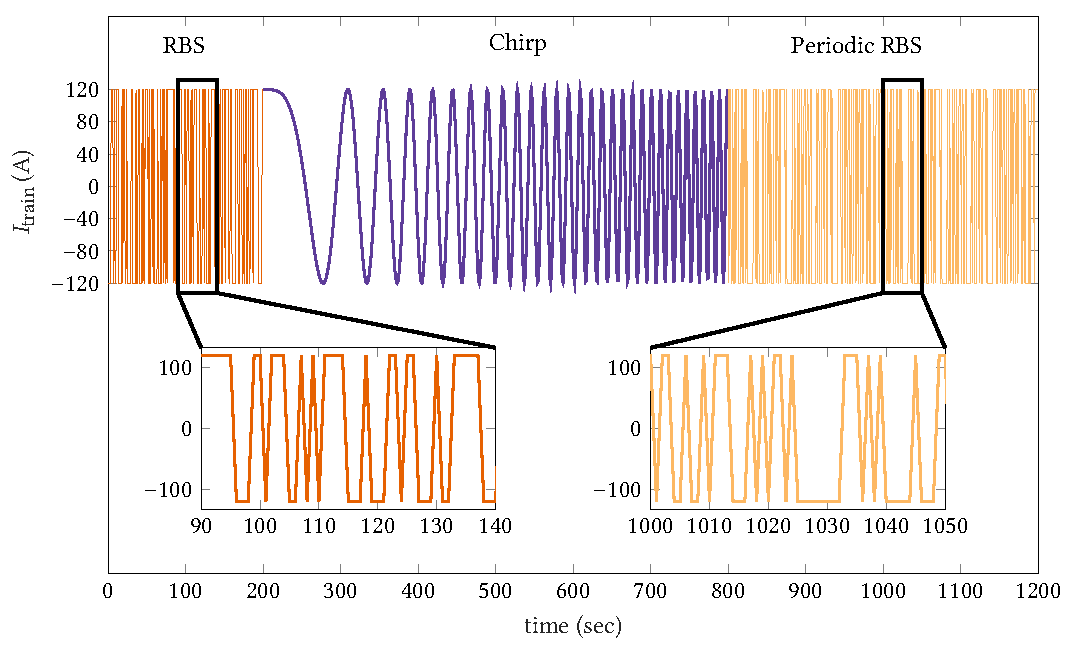
\includegraphics{sysid_train_input.pdf}
    \captionsetup{singlelinecheck=off}
    \caption[Input current profile used as the training set for system
    identification]{Input current profile used as the training set for system
    identification. The sequence consists of
    \begin{enumerate*}[label=\emph{\alph*})] \item a \glsfmtlong{rbs}, \item a
        chirp or swept cosine signal (0--\SI{100}{\milli\hertz}), and \item a periodic \glsfmtlong{rbs} \end{enumerate*} thereby
covering both low and high frequency spectra while incorporating the potential
to excite any periodic modes in the system to be identified.}
    \label{fig:sysidtrainingcurrent}
\end{figure}
Since not much prior  information is available about the poles  and zeros of the
electrolyte subsystem  in question, a wide  variety of special waveforms  with a
sampling interval of \SI{1}{\second} were used for the current perturbation used
in this system identification task. The specific input sequence consisted of
\begin{enumerate}
    \item \gls{rbs}\quad (0--\SI{199}{\second})
    \item `Chirp' \ie{} a swept cosine signal from 0--\SI{100}{\milli\hertz}\quad (200--\SI{799}{\second})
    \item Periodic \glsfmtlong{rbs} with a period of \SI{200}{\second} and 2 such periods\quad (800--\SI{1199}{\second})
\end{enumerate}
thereby helping to  obtain a wide-sense persistent excitation  signal. The swept
cosine  signal  is designed  to  excite  the low  frequency  (DC)  modes of  the
electrolyte subsystem and helps to capture the system's response to constant and
other systematically varying input profiles. The two \glspl{rbs} are intended to
target the poles and zeros of  the electrolyte subsystem that would typically be
excited  by  highly dynamic  input  profiles.  The  periodicity  in one  of  the
\glspl{rbs} was introduced  to draw out any hidden periodicity  or repeated real
poles  in the  system that  might  otherwise appear  to  be a  single pole.  The
presence  of both  low  and high  frequency frequency  spectra  in the  combined
training  set presents  a  high degree  of confidence  to  capture the  relevant
dynamics of the  electrolyte subsystem. The input current profile  used for this
system identification task is plotted in~\cref{fig:sysidtrainingcurrent}.

\subsection{Validation current profile}
For the  purposes of identification,  the \gls{p2d}  model is considered  as the
true system. First, the current profile from  the training set is applied to the
\gls{p2d} model. Its  simulation results, in particular,  the numerically solved
concentration values  at each spatially  discretised node  in each of  the three
regions per  time-step is then integrated  over the thickness of  the respective
regions  and multiplied  with their  respective porosities.  Thus the  number of
moles of \ch{Li^+}  per unit area in each of  the three regions $Q_{\text{e,}j}$
are obtained. Only  the quantities $Q_\text{e,n}$ and  $Q_\text{e,p}$ are chosen
as the outputs for system identification and a transfer function model is fitted
as per the evaluation procedure discussed in~\cref{subsubsec:actualsysid}.

As with  any classical  curve fitting  (numerical regression)  procedure, system
identification is also  prone to overfitting the training data.  In general, the
`best' transfer  function that identifies the  given system is the  lowest order
model that  can not  only minimize  the training error,  but also  minimizes the
error  on  a  previously  unseen  validation  dataset.  In  the  absence  of  an
independent validation dataset, the training error can be made arbitrarily small
by increasing  the number  of poles  and zeros of  the transfer  function models
without any  bounds. However, such a  model shall not have  truly identified the
dynamics of  the system  and shall  not generalise  well to  real-world datasets
outside  the training  realm. Hence,  having an  independent validation  current
profile for the task at hand is of paramount importance.

For the system identification task at  hand, the characteristic waveforms of the
validation profile were deliberately conjured to be differ vastly from that used
in training the model. The  validation profile consists of the following
sequence
\begin{enumerate}
    \item Periodic \gls{rgs} with 4 periods of \SI{200}{\second} each\quad (0--\SI{799}{\second})
    \item \gls{prbs} for emulating white noise, \ie{} with a flat power spectra
        across the frequency spectrum\quad (800--\SI{999}{\second})
    \item Multi-sine signal \ie{} a signal consisting of sinusoids at
        various fundamental frequencies added together\quad (1000--\SI{1199}{\second})
\end{enumerate}

Overall,  the validation  profile has  been designed  to cover  a wide  range of
frequencies  akin to  the  training  profile, but  differing  completely in  its
time-domain appearance.  The specific  validation current  profile used  in this
system identification is shown in~\cref{fig:sysidvalidationcurrent}.

\begin{figure}[!htb]
    \centering
    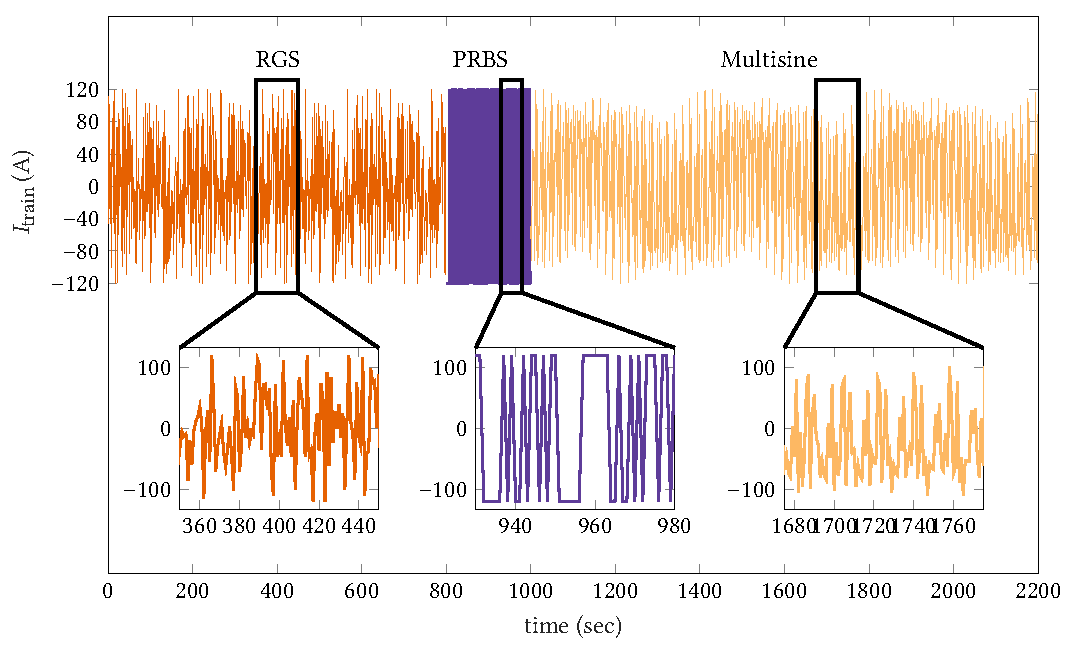
\includegraphics{sysid_validation_input.pdf}
    \captionsetup{singlelinecheck=off}
    \caption[Input current profile used as the validation set for system
    identification]{Input current profile used as the validation set for system
        identification. The sequence consists of
        \begin{enumerate*}[label=\emph{\alph*})]
            \item a \glsfmtlong{rgs},
            \item a \glsfmtlong{prbs}, and
            \item a multisine waveform
        \end{enumerate*}.
        The overall sequence  is intended to emulate the flat  power spectrum of
        white noise (with the \glsfmtshort{prbs}) and excite any poles and zeros
        within  3$\sigma$ spread  of the  \glsfmtshort{rgs} mean.  The multisine
        signal is  swept is composed  of sinusoids with  fundamental frequencies
        from \SI{100}{\milli\hertz}  up to the Nyquist  frequency. Its amplitude
        variation  across the  frequency spectrum  increases the  probability to
        capture the  system's modes that  were possibly missed by  the preceding
        two waveforms.
    }%
    \label{fig:sysidvalidationcurrent}
\end{figure}

\textsc{MATLAB} code  that can be used  to generate the training  and validation
input profiles is shown in~\cref{codesnippet:trainvalidsysidinput}.

\begin{listing}[!htbp]
\begin{minted}[mathescape,autogobble,bgcolor=mintedbg,escapeinside=||,texcomments=true]{matlab}
% Needs matlab's system identification toolbox
clear; close all; clc; format short g;
warning('off','Ident:dataprocess:idinput7'); % suppress sysid warnings
I_1C  = 60; % Amps
range = 2*[-I_1C I_1C]; % peak-peak swing is $\pm 2\text{C}=\SI{40}{\ampere}$
NumCh = 1; % no of channels (used by sysid toolbox for multichannel id)
Ts    = 1; % sampling interval

%% Random Binary Input Signal (RBS)
N  = 200; % samples per quantum of each waveform
u1 = idinput(N,'rbs',[],range); % 'idinput' from sysid toolbox
%% Chirp Signal (swept cosine)
t_chirp_start = 0;
t_chirp_end   = 3*N*Ts; %
t             = linspace(t_chirp_start,t_chirp_end,3*N);
f0            = 0;
f1            = 1e-1; % $f_1 = \SI{100}{\milli\hertz}$ is the max chirp frequency
u2            = max(range)*chirp(t,f0,t(end),f1)';
%% Periodic Random Binary Input Signal (Periodic RBS)
bin_seq_Period   = N; % seconds
bin_seq_Period_N = ceil(bin_seq_Period/Ts); % samples
bin_NumPeriod    = 2;
u3 = idinput([bin_seq_Period_N,NumCh,bin_NumPeriod],'rbs',[],range);
%% Random Guassian Signal (RGS)
rgs_Period         = N; % seconds
rgs_Period_samples = ceil(rgs_Period/Ts);
rgs_NumPeriod      = 4;
u4 = idinput([rgs_Period_samples,NumCh,rgs_NumPeriod],'rgs',[],range/2);
%% PseudoRandom Binary Signal (PRBS)
prbs_Period         = N; % seconds
prbs_Period_samples = ceil(prbs_Period/Ts);
u5                  = idinput(N,'prbs',[],range);
%% Multisine signal (sum of sines)
samples_per_Period = 2*N;
NumPeriod          = 3;
[u6,freq] = idinput([samples_per_Period 1 NumPeriod],'sine',[],range);

%% Split into training and validation data sets
I_load_train    = [u1;u2;u3];
I_load_validate = [u4;u5;u6];
\end{minted}
\caption{Generation of training and validation input current profiles in
\textsc{MATLAB}}
\label{codesnippet:trainvalidsysidinput}
\end{listing}

% Linearity and time-invariance

\section{Test for Linearity and Time Invariance}\label{sec:lticheck}
The      transfer     function      identification     techniques      mentioned
in~\cref{subsubsec:introblackboxsysid}   are  applicable  only   for   \gls{lti}
systems.  At the  first glance,  this seems  overly restrictive  for the  system
at  hand.  A lithium  ion  battery,  when  considered  as a  single  macroscopic
entity,  exhibits non-linear  characteristics,  particularly due  to the  strong
non-linearities in
\begin{enumerate*}[label=\emph{\alph*})]
    \item the Butler-Volmer reaction kinetics (see~\cref{eq:butlervolmer}), and
    \item the \glspl{ocp} of the two electrodes (see~\cref{eq:lcoUocpPos} and~\cref{eq:lcoUocpPos}).
\end{enumerate*}
However, since we are dealing with a much narrower scope \ie{} the systems under
consideration  are just  the two  sub-system entities  (one per  electrode) that
transform the  applied current at  a particular  time-step to the  overall moles
per  unit area  of  \ch{Li^+}  ions in  the  corresponding  electrode region  of
the  electrolyte at  that  same  instant. Therefore,  it  is  the linearity  and
time-invariance of these \emph{subsystems} that must be investigated.

\subsection{Time-invariance of the electrolyte time-evolution subsystems}\label{subsubsec:timeinvariance}
A  test  for time-invariance  is  prescribed  in  the  lecture notes  on  system
identification by  Plett~\cite{PlettECE5560_02}. The steps involved  therein are
reproduced here after  being suitably adapted to the notation  of the subsystems
at hand.
\begin{enumerate}
    \item Apply input $u_1(t) = I(t)$ to the system and measure the outputs $Q_{\text{e,n}_1}\!(t)$ and $Q_{\text{e,p}_1}\!(t)$.
    \item Apply a delayed version of the input by $\tau$ seconds \ie{} $u_2(t) = I(t-\tau)$ to the system and measure the outputs $Q_{\text{e,n}_2}\!(t)$ and $Q_{\text{e,n}_2}\!(t)$.
    \item If $Q_{\text{e,n}_2}\!(t)$ = $Q_{\text{e,n}_1}\!(t-\tau)$ and $Q_{\text{e,p}_2}\!(t)$ = $Q_{\text{e,p}_1}\!(t-\tau)$ for all possible delays $\tau$ as well as for choice of input signals $I(t)$, then the systems are time-invariant.
\end{enumerate}

For  the  systems   at  hand,  it  is  not  strictly   required  to  apply  this
prescriptive  test.  Unless a  fundamental  change  in the  underlying  reaction
phenomena/chemistry  occur that  alter the  performance over  time, systems  are
treated  as time-invariant.  Factors  that induce  time-dependent  shift in  the
behaviour of lithium ion batteries  are degradation phenomena such as thickening
of \gls{sei} layer  on the electrodes, dendrite growth or  mechanical fatigue in
electrodes  which in-turn  affect electrolytic  diffusion and  conductivity. Yet
another cause  of time-dependent  behavioural change is  the drift  in parameter
values. However, these  phenomena are typically one or mode  orders of magnitude
slower than  the \gls{p2d} dynamics\fxnote{citation needed}.  This separation of
time-scales  imply  that in  practice,  they  can  be decoupled  and  therefore,
separate  models can  be  identified  for the  faster  and  slower processes.  A
suitable model-blending approach  can then be considered to arrive  at cover all
processes across time-scales. Although the  concepts developed here for the fast
electrolyte dynamics can be suitably adapted to such slow phenomena, their study
falls outside  the scope of this  thesis and is  left as an exercise  for future
work.  Thus,  the overall  battery  system,  and  hence  by extension,  the  two
subsystems considered are deemed to  be time-invariant. However, in the interest
of  completeness, this  author  systematically applied  the aforementioned  test
procedure  with every  combination arising  from  the choice  of ten  time-delay
values and the following six current profiles ---
\begin{enumerate*}[label=\emph{\alph*})]
    \item constant current 1C discharge,
    \item constant current 3C discharge,
    \item constant current 1C charge,
    \item \gls{udds} input profile with peak amplitude of 3C,
    \item training profile used in system identification (see~\cref{fig:sysidtrainingcurrent}), and
    \item validation profile used in system identification (see~\cref{fig:sysidvalidationcurrent}).
\end{enumerate*}
Finally,  these tests  were  repeated for  a choice  of  five different  initial
\glspl{soc}   ---   \SI{90}{\percent},   \SI{70}{\percent},   \SI{50}{\percent},
\SI{30}{\percent}  and \SI{10}{\percent}\footnote{\label{fn:socstart}The  number
of  moles  of  \ch{Li^+} per  unit  area  in  the  electrolyte does  not  depend
on  the  electrode's \glsfmtshort{soc}.  However,  different  starting point  of
\glsfmtshort{soc}s were considered  to have a wide variety in  the length of the
recorded  data until  cut-offs  were hit.  \eg{}  starting at  \SI{90}{\percent}
\glsfmtshort{soc} could  mean that  for a  current spike  early in  the profile,
upper  cut-off voltage  shall be  hit  sooner leaving  a smaller  set of  logged
simulation data.}.

\begin{figure}[!htb]
    \centering
    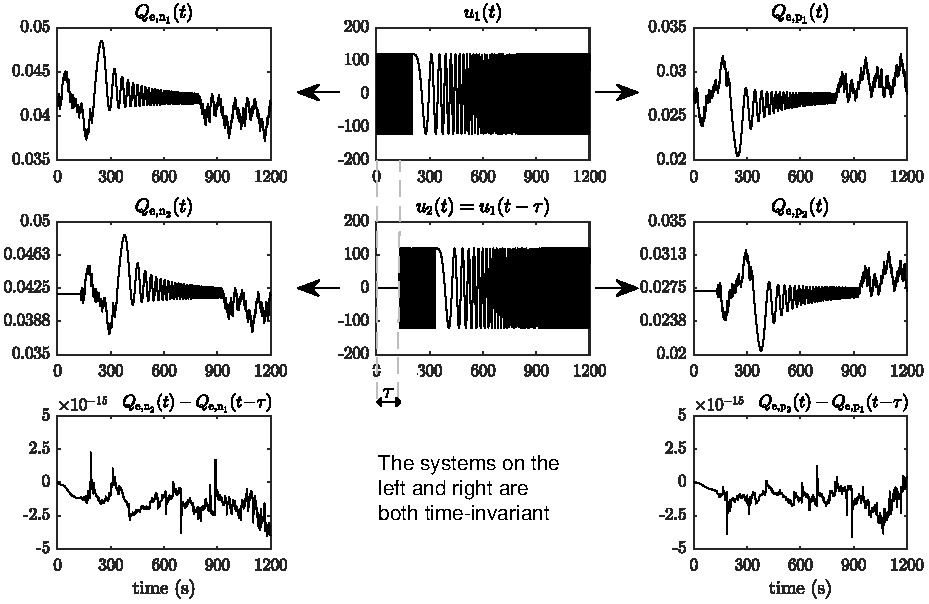
\includegraphics[width=\textwidth]{time_invariance.pdf}
    \caption[Demonstration of time-invariance of $Q_\text{e,n}(t)$ and
    $Q_\text{e,p}(t)$ subsystems]{Demonstration of time-invariance of the
        subsystems considered. The applied current profile $u_1(t)$ is the
        system identification training sequence
        from~\cref{fig:sysidtrainingcurrent} (top row of the central column).
        The top left plot shows the response $Q_{\text{e,n}_1}\!(t)$, while that
        on the top right shows $Q_{\text{e,p}_1}\!(t)$. The second row of the
        middle column shows the same input sequence delayed by $\tau =
        \SI{130}{\second}$. Application of this current profile $u_2(t) =
        u_1(t-\tau)$ results in the outputs $Q_{\text{e,n}_2}\!(t)$ and
        $Q_{\text{e,p}_2}\!(t)$ to its left and right respectively. Subtracting
        these from the correspondingly delayed versions of the original outputs
        result in zero residuals, thereby proving time-invariance of these
        subsystems. The jitter shown in the bottom row of plots is
        $\mathcal{O}(10^{-15})$ in magnitude and are due to the numerical
        roundoffs that occur when operating close to the noise floor of the
    machine's floating point units.}%
\label{fig:timeinvariance}
\end{figure}
% The outputs $Q_\text{e,n}$ and $Q_\text{e,p}$ are shown to the left and right of the applied input.

\Cref{fig:timeinvariance}  demonstrates the  time-invariance  of the  subsystems
considered  at an  initial \gls{soc}  of \SI{50}{\percent}  for a  time-delay of
\SI{130}{\second}  using  the  highly  dynamic  system  identification  training
sequence  that  was synthesised  by  this  thesis  author. The  applied  current
profile  $u_1(t)$  (top  row  of   the  central  column)  produces  the  outputs
$Q_{\text{e,n}_1}\!(t)$ and  $Q_{\text{e,p}_1}\!(t)$ shown  in the top  left and
top right  plots respectively. When the  delayed version of this  input sequence
${u_2(t) = u_1(t-\tau)}$  (middle row, middle column) is applied,  it results in
the outputs $Q_{\text{e,n}_2}\!(t)$ and  $Q_{\text{e,p}_2}\!(t)$ to its left and
right respectively. Following the steps of the test procedure, subtracting these
outputs from the correspondingly delayed versions of their original counterparts
result in  zero residuals, thereby  proving time-invariance of  these subsystems
under these representative test conditions. The residual sequences in the bottom
row of plots are of $\mathcal{O}(10^{-15})$ and arise due to numerical roundoffs
that occur  when operating close  to the noise  floor of the  machine's floating
point units.

Similar to  the case demonstrated  here, all  tests for time-invariance  for all
permutations of  the chosen operating  conditions passed successfully  \ie{} the
delayed  version of  the original  output  signals accurately  matched with  the
responses  to  the corresponding  delayed  input  (down to  machine  precision),
thereby confirming the time-variance of  the subsystems considered in the system
identification problem, which enables us to proceed further.


\subsubsection*{Linearity   analysis    of   the    time-evolution   electrolyte
subsystems}\label{subsubsec:linearityanalysis}

In the analyses of linearity of systems, it is a recommended practice to de-bias
the output and input quantities about their mean operating conditions. The input
signal in  this case,  is the  applied load  current $I(t)$,  which can  be both
positive (during  discharge) and negative  (during charge). Although  in typical
drive-cycles there  is a net  discharge, the value  of the mean  applied current
differs across  drivecycles. Furthermore, drivecycles are  merely representative
profiles and therefore, in real-world operation, the cell needs to be treated as
being equally  probable for being  subjected charged and discharged.  Hence, the
mean  of the  input signal  is taken  as zero,  which eliminates  any de-biasing
requirements.

For  the output  signals  though, bias  values can  be  clearly identified.  The
overall number of moles of \ch{Li^+} per unit area in any region within the cell
cannot be physically negative. Even though  under high C-rates, ion depletion at
localised  spatial  locations (such  as  the  current collectors)  is  certainly
possible, the entire thickness of any region cannot become devoid of ions at any
point in time  since the cell shall  instantaneously cease to work.  Thus, for a
typical well-designed  cell operating within the  manufacturer prescribed C-rate
limits, the output  signals under consideration operate in a  small window about
their initial values. In the author's  simulations, even at $\pm$5C, the overall
number of moles  of \ch{Li^+} in any  cell region exhibited a  maximum change of
less than \SI{15}{\percent}  from its initial value. Thus,  the de-biased output
variables  for  system  identification, $\widetilde{Q}_{\text{e,}j}(t)$  can  be
obtained  by subtracting  their  respective  initial values  $Q_{\text{e,}j}(0)$
(see~\cref{eq:Qeninit} and~\cref{eq:Qepinit}) from $Q_{\text{e,}j}(t)$.
\begin{align}
    \widetilde{Q}_\text{e,n}(t) & = {Q}_\text{e,n}(t) - {Q}_\text{e,n}(0) \\
    \widetilde{Q}_\text{e,p}(t) & = {Q}_\text{e,p}(t) - {Q}_\text{e,p}(0)
\end{align}
which   implies   that   the   transfer  functions   to   be   identified   have
to   be   modified    to   be   $\frac{\widetilde{Q}_\text{e,n}(s)}{I(s)}$   and
$\frac{\widetilde{Q}_\text{e,p}(s)}{I(s)}$  respectively. This  does not  affect
the time-invariance proved  in~\cref{subsubsec:timeinvariance} since the initial
values $Q_{\text{e,}j}(0)$ are merely constants and hence not time-dependent.

Similar     to      the     test      for     time      invariance     described
in~\cref{subsubsec:timeinvariance}, a  test for linearity is  also prescribed in
the lecture notes on  system identification by Plett~\cite{PlettECE5560_02}. The
steps involved therein  are reproduced here after being suitably  adapted to the
notation of the subsystems at hand. This is essentially a recipe for testing the
superposition principle.
\begin{enumerate}
    \item Apply input profile $I_1(t)$ to the system and obtain outputs $\widetilde{Q}_{\text{e,n}_1}\!(t)$ and $\widetilde{Q}_{\text{e,p}_1}\!(t)$.
    \item Apply a different profile $I_2(t)$ to the system and obtain outputs $\widetilde{Q}_{\text{e,n}_2}\!(t)$ and $\widetilde{Q}_{\text{e,n}_2}\!(t)$.
    \item Now apply an input profile $I_3(t) = \alpha I_1(t) + \beta I_2(t)$ and obtain a corresponding set of outputs $\widetilde{Q}_{\text{e,n}_3}\!(t)$ and $\widetilde{Q}_{\text{e,n}_3}\!(t)$.
    \item If $\widetilde{Q}_{\text{e,n}_3}\!(t)$ = $\alpha\, \widetilde{Q}_{\text{e,n}_1}\!(t) + \beta \, \widetilde{Q}_{\text{e,n}_2}\!(t)$ and $\widetilde{Q}_{\text{e,p}_3}\!(t)$ = $\alpha\, \widetilde{Q}_{\text{e,p}_1}\!(t) + \beta \, \widetilde{Q}_{\text{e,p}_2}\!(t)$ for all possible $\{\alpha,\beta\}$ as well as for choice of input signals $\{I_1(t),I_2(t)\}$, then the systems are linear.
\end{enumerate}

Similar  to   the  time-invariance  test,   the  same  set  of   five  different
initial  \glspl{soc}\ref{fn:socstart} ---  \SI{90}{\percent}, \SI{70}{\percent},
\SI{50}{\percent},  \SI{30}{\percent} and  \SI{10}{\percent},  was retained  for
these linearity tests.  For each test run, a pseudo-random  number generator was
used to  select the values  of $\{\alpha,\beta\}$ from  the set of  real numbers
$\mathbb{R}$ (not restricted to the set  of integers $\mathbb{Z}$) in the closed
interval spanning  $[-1.25,1.25]$. Negative values  are acceptable for  both the
scaling coefficients since the resulting  composite input $I_3(t)$ can be either
positive or  negative. The composite  signal $I_3(t)$  was obtained by  taking a
random combination of any two of the following current profiles ---
\begin{enumerate*}[label=\emph{\alph*})]
    \item constant current 1C discharge,
    \item constant current discharge at C/5,
    \item constant current 1C charge,
    \item constant current charge at C/5,
    \item training profile used in system identification (see~\cref{fig:sysidtrainingcurrent}), and
    \item validation profile used in system identification (see~\cref{fig:sysidvalidationcurrent}).
\end{enumerate*}

The  scaling  factors  $\alpha$  and   $\beta$  were  restricted  to  the  range
$[-1.25,1.25]$ in consideration of limiting the peak applied current to within a
\pm 5C  window ---  the operating  condition for most  \glspl{bev}, so  that the
isothermal assumption for the model shall remain valid. This peak current corner
case occurs when the pseudo-random generator chooses both scaling factors at the
selected range's limits for the 1C constant current discharge or charging cases.
The limited  range of the  scaling factors are also  motivated by the  fact that
most real-world systems remain linear only within a certain operating window. In
particular, care  must be taken to  ensure that the cell's  \gls{soc} during the
linearity test  remains within  its physical limits  for any  initial \gls{soc}.
Furthermore, localised  saturation or depletion  of ions for  extended durations
must be avoided. Hence  it can be concluded that, with the  chosen range for the
scaling  factors,  if  the  two subsystems  under  consideration  remain  linear
everywhere below  a peak  current of  \pm 5C  in the  isothermal case,  then the
linearity  tests are  considered as  passed.  Future extensions  to undertake  a
temperature-dependent  system  identification  exercise can  potentially  use  a
first-order Taylor  expansion about this  operating window. The  discussion thus
far has fully established all the conditions for conducting the for linearity.

\begin{figure}[!htb]
    \centering
    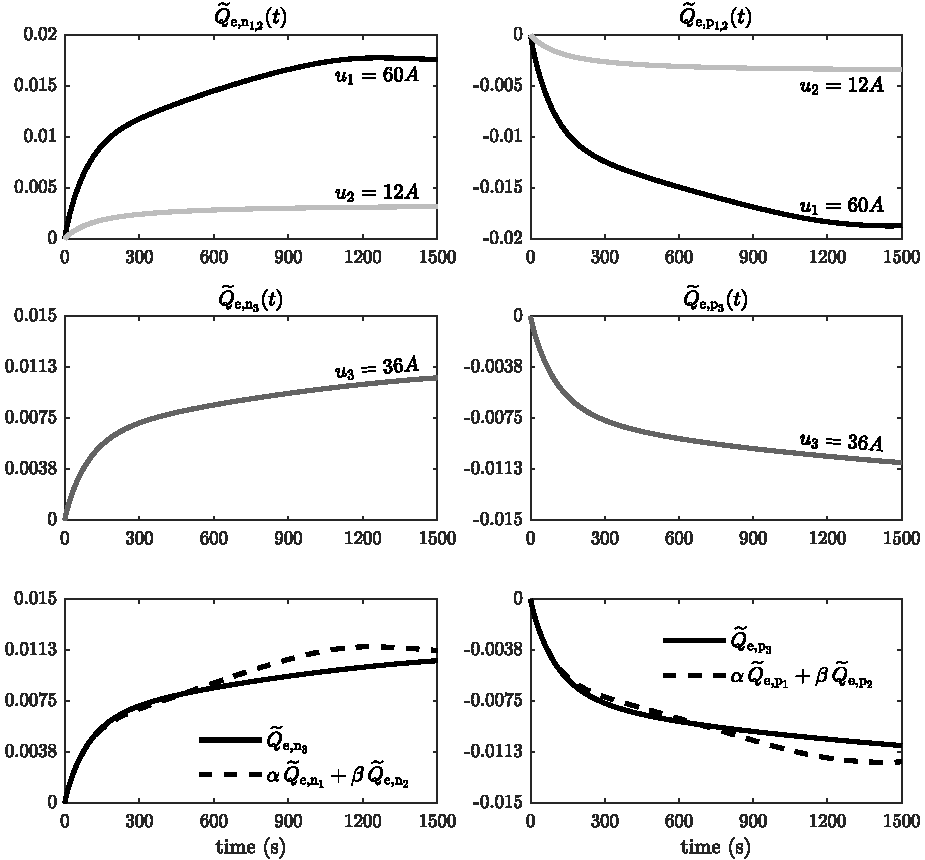
\includegraphics[width=\textwidth]{linearity_proof}
    \caption[Illustration of linearity test for the
    \protect{$\widetilde{Q}_{\text{e,n}}$} and
    \protect{$\widetilde{Q}_{\text{e,p}}$} subsystems]{Illustration of one
        instance of linearity tests for the subsystems under consideration. For
        this visualisation, constant current inputs are used throughout. The top
        row of plots shows $\widetilde{Q}_{\text{e,n}}$ and
        $\widetilde{Q}_{\text{e,p}}$ for two input currents $I_1(t) =
        \SI{60}{\ampere}$ and $I_2(t) = \SI{12}{\ampere}$ \ie{} discharge with
        1C and C/5 currents respectively. The second row of plots shows
        $\widetilde{Q}_{\text{e,n}_3}$ and $\widetilde{Q}_{\text{e,p}_3}$  for
        $I_3 = \SI{36}{\ampere}$, where $I_3 = \alpha I_1 + \beta I_2$ with
        $(\alpha,\beta) = (1,-2)$. The last row of plots overlays these
        quantities with the manually computed linear combination of their two
        preceding responses. Had these sequences overlapped exactly, the systems
        would have been exactly linear. Despite exhibiting deviations over the
        considered horizon, the transient responses in both electrode regions do
        follow the superposition principle. Even past the transient, maximum
        error in both cases is an order of magnitude lower than the individual
        outputs. Hence, the two systems are deemed to be \emph{approximately}
        linear.
    }%
    \label{fig:linearity}
\end{figure}

\Cref{fig:linearity}  illustrates  one  instance  of a  linearity  test  wherein
constant  currents  and  integer  scaling  factors are  used  for  the  sake  of
illustration.  The  plots   in  the  left  column  deal   with  the  electrolyte
time-evolution  subsystem  in  the  negative electrode  region.  Similarly.  the
plots  in  the  right  column  deal with  the  corresponding  subsystem  in  the
positive electrode region.  A discharge current of 1C  \ie{} \SI{60}{\ampere} is
first  applied  and  the  corresponding  outputs  $\widetilde{Q}_{\text{e,n}_1}$
and   $\widetilde{Q}_{\text{e,p}_1}$  are   obtained.   Secondly,  a   discharge
current   of   C/5   \ie{}   is    applied   and   the   corresponding   outputs
$\widetilde{Q}_{\text{e,n}_2}$ and  $\widetilde{Q}_{\text{e,p}_2}$ are obtained.
These set of responses are plotted  in the top row of~\cref{fig:linearity}. Now,
a  third  value  of  input  current $I_3$,  computed  as  a  linear  combination
of  the  previous  input  currents  \ie{}  $I_3 =  \alpha  I_1  +  \beta  I_2  $
is  applied.  For  illustrative  purposes, the  integer  set  $(\alpha,\beta)  =
(1,-2)$  was  chosen  for  the   scaling  coefficients,  which  implies  $I_3  =
\SI{12}{\ampere}$. The corresponding  outputs $\widetilde{Q}_{\text{e,n}_3}$ and
$\widetilde{Q}_{\text{e,p}_3}$ are  plotted in the  middle row. As per  the test
for linearity,  if these signals are  equal to the signal  generated by manually
computing the linear  combination of the preceding two outputs,  then the system
is linear.

The   plots   in  the   third   row   show  $\widetilde{Q}_{\text{e,n}_3}$   and
$\widetilde{Q}_{\text{e,p}_3}$ overlaid with their respective linear combination
signals. In  the case  of the  subsystem in the  negative electrode  region, the
transient performance matches  precisely until \approx\SI{450}{\second}, whereas
that in the positive electrode region exhibits a good matching for approximately
the  first  \SI{250}{\second}.  However,  for the  horizon  considered  the  two
overlaid plots do not overlap exactly.  Hence, the systems are not truly linear.
However, the exhibited  behaviour is quite close to linearity,  with the maximum
absolute  error  in each  region,  even  outside  the initial  transient,  being
$\mathcal{O}(10^{-4})$  --- an  order  of magnitude  lower  than its  individual
components.  This behaviour  was exhibited  for all  test instances  considered.
Considering  that for  dynamic  simulation runs,  the  transient performance  is
paramount  to  the good  performance  of  the  model,  in conjunction  with  the
aforementioned  low error  metric,  these  subsystems can  be  considered to  be
\emph{approximately} linear.


% Discussion of identification choices here

\subsection{Identification Methodology and Governing Equations}\label{subsubsec:actualsysid}
\subsection{Performance of Final Model}
\section{Embedding into SPM and final results for composite system}

% Assumed transfer function model. Test results within the model itself
% Test results for electrolyte ce (subsection)
% test results for full system (final section)

% mention in introduction where code snippets are given


% \section{Brief Introduction to System Identification}\label{subsec:introsysid}
% % -*- root: ../main.tex -*-
%!TEX root = ../main.tex
% this file is called up by main.tex
% content in this file will be fed into the main document
% vim:textwidth=80 fo=cqt


An in-depth  coverage of the topic  of system identification is  well beyond the
scope of  this thesis.  However, keeping  in mind the  interests of  the battery
modelling community  who might not be  familiar with this subject  area, a brief
overview of the core ideas that  are essential for tackling the specific problem
at hand is  presented. For readers further interested in  this topic, the author
suggests the textbook by  Ljung~\cite{Ljung1999} for a comprehensive theoretical
treatment of the foundation topics in system identification.

System identification aims  to provide a mathematical model  of the input-output
mapping  of the  system\footnote{The precise  definition of  what constitutes  a
`system' is detailed  in Ljung's textbook. However, for  all practical purposes,
in this  thesis the word `system'  stands for any unknown  entity whose terminal
behavioural model  is being  sought for ---  primarily from  input-output data.}
under consideration. The three categories of system identification are:


\begin{enumdescriptnum}[leftmargin=!,itemsep=1ex,labelwidth=\widthof{$\symbf{\text{brugg}_j}\ \scriptstyle (\times 3)$abc}
    ,partopsep=0pt
    ,topsep=0pt
    ]

\item[White  box] wherein  underlying physical  equations are  completely known.
The  numerical value  of  coefficients of  governing equations  are  then to  be
parametrised from input-output data.

\item[Black box]  wherein no  governing equations are  available for  the system
under  consideration. The  model formulation  is facilitated  by a  rich set  of
system theory  which proceeds by exciting  the system with input  waveforms with
certain desirable  properties and correlating characteristics  from the response
to draw  conclusions about viable  mathematical structures capable  of emulating
the terminal behaviour of the system  under generalised inputs. Black box system
identification was employed for the specific problem under consideration in this
thesis and hence all future descriptions will pertain to this class.

\item[Grey box] is a hybrid of the  two approaches wherein a part of the model's
governing  physics is  known  a priori  \eg{} the  structure  of a  well-defined
subsystem  that is  part  of a  large,  complex  system may  be  known ahead  of
time,  where the  task  is  to characterise  the  full  system. Grey box  system
identification tasks can  often be reduced to a single  sub-problem of black box
system  identification  by  removal  of  the known  physics  and  tackling  them
separately.

\end{enumdescriptnum}



% \section{Overview of Black Box System Identification}\label{sec:introblackboxsysid}
% % -*- root: ../main.tex -*-
%!TEX root = ../main.tex
% this file is called up by main.tex
% content in this file will be fed into the main document
% vim:textwidth=80 fo=cqt

Black-box system identification techniques are composed of the following ---
\begin{enumerate*}[label=\emph{\alph*})]
     \item non-parametric methods, and
     \item parametric methods.
 \end{enumerate*}

\subsection{Non-parametric methods}
Non-parametric methods do not seek  a pre-assumed mathematical structure for the
system. They  aim to  directly estimate  the very  kernel of  what characterises
every system \viz{}  the Markov parameters in the time-domain  and the \gls{frf}
in the frequency domain, thereby requiring \emph{infinite} number of data points
for  their representation.  Major non-parametric  system identification  methods
include:
\begin{itemize}[topsep=0pt]
    \item Identification in time domain
        \begin{itemize}

            \item Direct  estimation of the system's  Markov parameters through
                statistical correlation of its response to an unit-pulse input.

        \end{itemize}
    \item Identification in frequency domain,  \ie{} of the \gls{frf}
        \begin{enumerate}

            \item   Direct   estimation    through   input-output   statistical
                cross-correlation.

            \item  \gls{etfe} using \glspl{dft} of input and output sequences.

            \item  Smoothed periodogram estimates using Welch's method.

            \item  Blackman-Tukey  Estimate   using  standard  filter
                windows  in digital  signal processing  (such as  Hamming, Hanning,
                Bartlett, Boxcar etc.).

        \end{enumerate}
\end{itemize}

\subsection{Parametric methods}
Parametric  methods aim  to fit  specific input-output  data to  some family  of
well-known  mathematical constructs  that are  well-known and  widely applicable
to  a  large  variety  of  inputs.   It  is  important  to  recognise  that,  in
contrast to white-box system identification, the salient coefficients/properties
of  these  mathematical structures  \emph{do  not,}  in  any way  correspond  to
physical properties of  the system under consideration.  Major parametric system
identification methods use:
\begin{itemize}
    \item Transfer-function based frequency domain model structures
        \begin{enumerate}
            \item \gls{oe} model
            \item \gls{arx} model
            \item \gls{armax} model
            \item Box-Jenkins (BJ) model
        \end{enumerate}
    \item State-space time-domain model structures
        \begin{enumerate}
            \item Ho-Kalman realisation
            \item \gls{era} realisation
            \item Deterministic and stochastic \emph{subspace} structures
        \end{enumerate}
\end{itemize}

\subsection{Investigation of suitable system identification methodology}
% \subsubsection*{Ill-suitability of non-parametric methods}
Among   the   various   system    identification   techniques   mentioned,   the
non-parametric   methods    have   some    serious   drawbacks.    As   outlined
in~\cref{subsec:sysidbackground}, the author is inspired  by the trait of having
a pre-assumed model structure that  brought the baseline quadratic approximation
closer to a successful realisation. The non-parametric methods do not conform to
this philosophy. Furthermore, the requirement of infinite number of data samples
in order to fully quantify the system dampens its feasibility for implementation
in  resource  constrained  environments.  The  author is  of  the  opinion  that
resorting  to truncation  of  the  characteristic sequence  shall  only yield  a
sub-optimal solution. Hence non-parametric methods are ruled out for applying to
the task at hand.

While  parametric state-space  identification is  a feasible  alternative, these
methodologies are tedious and error-prone.  For instance, applying the Ho-Kalman
algorithm requires construction of large-sized Block-Hankel matrices followed by
a  \gls{svd} operation.  The  \gls{era}  uses the  identical  set of  operations
of  the  Ho-Kalman   procedure,  except  that  certain  blocks   in  the  Hankel
matrices  are chosen  at  random  for deletion  for  obtaining better  estimates
in  low  \gls{snr} environments  and  for  capturing slowly  decaying  phenomena
with  long time  constants. The  subspace methods  are mathematically  involved,
requiring  a  profound  understanding  of  concepts  from  linear  algebra  such
as  projections  to orthogonal  subspaces.  The  system under  consideration  is
presented in~\cref{sec:introtoplant} and after linearity considerations, refined
in~\cref{subsec:linearityanalysis}. It is composed of two independent \gls{siso}
subsystems.  However,   the  inflection  point  in   the  complexity-performance
trade-off  in state-space  identification  is achieved  only  when dealing  with
\gls{mimo} systems that suggest strong  cross-coupling among its internal states
or  at least  some degree  of  coupling among  the various  inputs and  outputs.
Furthermore, the impulse  responses of the system(s) under  consideration do not
have long tails since they are characterised by relatively short time constants.
Owing to these  reasons, it was decided that state  space identification methods
shall not be adopted here.

Owing to a  cornucopia of well-established technical  know-how readily available
in the systems  engineers toolkit, transfer function based  model structures are
naturally amenable  for control-oriented applications. However,  there exists an
apparent discrepancy to  its usage for this case, that  must be addressed first.
Transfer  function methods  are  a  frequency domain  technique  and hence,  the
resulting model  descriptions have  mathematical structures  radically different
from the time-domain model equations  of the conventional \gls{spm} within which
they are  to be embedded. This  conundrum is resolved by  closely inspecting the
model's scope  and its tractability for  conversion to time domain  as explained
next.

It  is  worth remembering  that,  as  per~\cref{subsec:freqdomainroms}, for  the
reduced order  modelling of the  \emph{entire cell}, all frequency  domain model
groups were considered  as out of scope  of this thesis specifically  due to the
overhead  of conversion  from frequency  to time  domain for  implementation and
other associated difficulties. The blanket exclusion nature of this statement is
to be revisited considering the specific scope  of the problem at hand. The body
of literature  on frequency  domain \glspl{rom} discuss  obtaining physics-based
\emph{transcendental}   transfer   functions  for   \emph{all}   electrochemical
quantities  of the  coupled  \gls{pdae} system  of~\cref{tbl:dfneqns} through  a
top-down approach.  However, the frequency domain  system identification methods
are concerned with  obtaining standard \emph{rational} transfer  functions for a
much narrower  scope \viz{}  the time-evolution  subsystem, through  a bottom-up
approach.  Such  rational transfer  functions  are  to obtained  for  \gls{siso}
systems for which an approximation-free  effortless conversion already exists in
classical control theory and is  presented in~\cref{sec:actualsysid}. In view of
their  overwhelming  simplicity  and  familiarity to  control  engineers,  after
considering these  arguments that circumvent  their only apparent  impediment to
adoption, \emph{transfer  function} based  system identification was  chosen for
tackling the problem at hand. The  steps leading to the identification procedure
is presented next.


% might possibly have to promote into its own detailed subsection



% \section{Introduction to Electrolyte Time-Evolution Subsystems}\label{sec:introtoplant}
% % -*- root: ../main.tex -*-
%!TEX root = ../main.tex
% this file is called up by main.tex
% content in this file will be fed into the main document
% vim:textwidth=80 fo=cqt

The                  first                 order~\glspl{ode}                  of
\crefrange{eq:negliionmolesquadratic}{eq:posliionmolesquadratic} in the baseline
quadratic  approximation  model  for   electrolyte  concentration  describe  the
time-evolution of the overall number of moles  of \ch{Li^+} in each of the three
regions of the cell $Q_{\text{e,}j}$.  Through system identification, the author
seeks  to obtain  the two  rational transfer  functions of  $Q_\text{e,neg}$ and
$Q_\text{e,pos}$  to the  applied current  $I$  in the  frequency domain,  \ie{}
$\frac{Q_\text{e,n}(s)}{I(s)}$ and $\frac{Q_\text{e,p}(s)}{I(s)}$.  Based on the
\gls{dfn} model,  the total moles of  \ch{Li^+} per unit area  in the separator,
$Q_\text{e,s}$ is  not a function  of the exogenous applied  current. Therefore,
the baseline  quadratic approximation  \gls{ode} is  retained for  computing its
time-evolution.



% \section{Design of Persistent Excitations}\label{sec:persistentexcitation}
% % -*- root: ../main.tex -*-
%!TEX root = ../main.tex
% this file is called up by main.tex
% content in this file will be fed into the main document
% vim:textwidth=80 fo=cqt

In order  to successfully apply  any system identification technique,  the input
signal must be carefully  designed to be persistently exciting~\cite{Ljung1999}.
Narendra and Annaswamy~\cite{Narendra1984,Narendra1987}  were among the earliest
researchers  to provide  a detailed  treatment  of the  desirable properties  of
persistent excitation and their implication to the quality of the identification
output. A  practical method to achieve  persistent excitation is to  subject the
system under  consideration to  a sequence  of well-characterised  input signals
that  are  capable of  exciting  its  hypothesised  modes.  For this  task,  the
author  of this  thesis  chose  to use  the  data-quality  guidance provided  by
The~Mathworks~Inc.~\cite{mathworkssysid}\ and performed  an iterative refinement
until the identification procedure resulted in a generalisable model.

Before discussing the shape characteristics of the input sequence, its magnitude
must be established.  The various specially prepared input  sequence families do
not  share a  common definition  for their  magnitudes. A  guiding principle  in
system  identification is  that  it  is important  to  have  the input  signal's
magnitude  to  be  representative  of standard  operating  conditions.  Although
standardised  drive  cycle  profiles  are  available,  from  which  a  speed  to
current mapping  can be  performed, it  is impossible to  predict a~priori, the
specific  amplitudes of  currents  that  the cell  may  undergo under  real-life
load  conditions.  Without  further  deterministic information,  the  author  of
this  thesis  chose to  interpret  magnitude  as  being  the peak  amplitude  of
the  input  current  profile. As  seen  in \cref{fig:uddssimp2dspmresults},  the
representative  \gls{udds}  drivecycle  input  profile  corresponds  to  a  peak
of  3C \ie{}  \SI{180}{\ampere}.  Following the  standard  principles of  system
identification, it is desirable  for the inputs to the system  to lie along some
measure  of  central tendency.  This  is  to  enable  the identified  system  to
generalise well \ie{} not deviate too far  from the truth when subject to inputs
that are far away from the central  measure. Yet another consideration is not to
saturate the identified model by choosing input magnitude to be too close to the
peak of  the expected  operating range. Taking  into account  all aforementioned
considerations, the  peak amplitude of the  input current was fixed  at 2C \ie{}
\ordfrac{2}{3} of the \gls{udds} profile's peak current amplitude.

\subsection{Training current profile}\label{subsec:trainingprofile}

Since not much prior  information is available about the poles  and zeros of the
electrolyte subsystem(s)  in question, a wide  variety of special waveforms  with a
sampling interval of \SI{1}{\second} were used for the current perturbation used
in this system identification task. The specific input sequence consisted of
\begin{enumerate}
    \item \gls{rbs}\quad (0--\SI{199}{\second})
    \item `Chirp' \ie{} a swept cosine signal from 0--\SI{100}{\milli\hertz}\quad (200--\SI{799}{\second})
    \item Periodic \glsfmtlong{rbs} with a period of \SI{200}{\second} and 2 such periods\quad (800--\SI{1199}{\second})
\end{enumerate}
thereby  helping  to  obtain  a  wide-sense  persistent  excitation.  The  swept
cosine  signal  is designed  to  excite  the low  frequency  (DC)  modes of  the
electrolyte subsystem and helps to capture the system's response to constant and
other systematically  varying input profiles.  The two \glspl{rbs}  are intended
to  target  the  poles  and  zeros  of  the  electrolyte  subsystem  that  would
typically be  excited by highly dynamic  input profiles. The periodicity  in one
of  the  \glspl{rbs} was  introduced  to  draw out  any  repeated  real pole  or
complex  conjugate  poles  poles  in  the system  that  might  otherwise  appear
to  be  a  single real  pole.  The  presence  of  both low  and  high  frequency
frequency  spectra in  the  combined  training set  presents  a  high degree  of
confidence to  capture the relevant  dynamics of the electrolyte  subsystem. The
input  current profile  used  for  this system  identification  task is  plotted
in \cref{fig:sysidtrainingcurrent}.

\begin{figure}[!htbp]
    \centering
    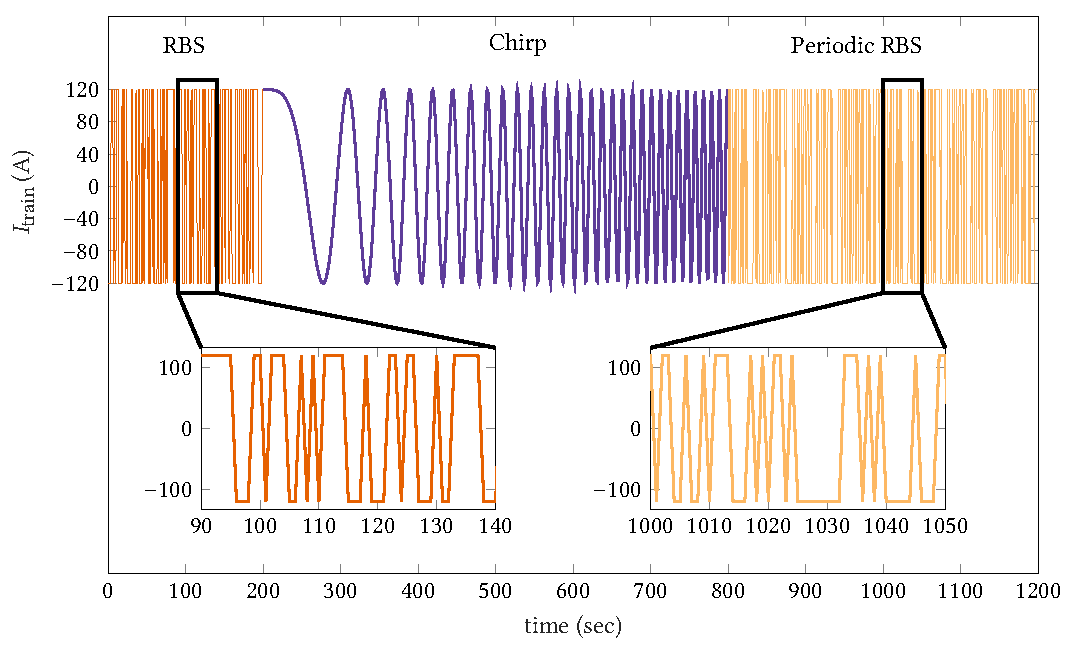
\includegraphics{sysid_train_input.pdf}
    \captionsetup{singlelinecheck=off}
    \caption[Input current profile used as the training set for system
    identification]{Input current profile used as the training set for system
    identification. The sequence consists of
    \begin{enumerate*}[label=\emph{\alph*})] \item a \glsfmtlong{rbs}, \item a
        chirp or swept cosine signal (0--\SI{100}{\milli\hertz}), and \item a periodic \glsfmtlong{rbs} \end{enumerate*} thereby
covering both low and high frequency spectra while incorporating the potential
to excite any periodic modes in the system to be identified.}
    \label{fig:sysidtrainingcurrent}
\end{figure}

\subsection{Validation current profile}

For the  purposes of identification,  the \gls{p2d}  model is considered  as the
true system. First, the current profile from  the training set is applied to the
\gls{p2d} model.  Its simulation results,  in particular the  numerically solved
concentration values  at each spatially  discretised node  in each of  the three
regions per time-step is integrated over the thickness of the respective regions
and multiplied with their respective porosities to obtain the number of moles of
\ch{Li^+} per unit area in each  of the three regions $Q_{\text{e,}j}$. Only the
quantities  $Q_\text{e,n}$ and  $Q_\text{e,p}$  are chosen  as  the outputs  for
system  identification and  a  transfer  function model  is  fitted  as per  the
evaluation procedure discussed in \cref{sec:actualsysid}.

As with  any classical  curve fitting  (numerical regression)  procedure, system
identification is also  prone to overfitting the training data.  In general, the
`best' transfer  function that identifies the  given system is the  lowest order
model that not  only minimizes the training error, but  also minimizes the error
on a  previously unseen  validation dataset.  In the  absence of  an independent
validation  dataset,  the  training  error  can be  made  arbitrarily  small  by
increasing the number of poles and zeros of the transfer function models without
any bounds. However,  such a model shall not have  truly identified the dynamics
of the system  and shall not generalise well to  real-world datasets outside the
training realm. Hence, having an  independent validation current profile for the
task at hand is of paramount importance.

For the system identification task at  hand, the characteristic waveforms of the
validation profile were deliberately conjured to be differ vastly from that used
in training the model. The  validation profile consists of the following
sequence
\begin{enumerate}
    \item Periodic \gls{rgs} with 4 periods of \SI{200}{\second} each\quad (0--\SI{799}{\second})
    \item \gls{prbs} for emulating white noise, \ie{} with a flat power spectra
        across the frequency spectrum\quad (800--\SI{999}{\second})
    \item Multi-sine signal \ie{} a signal consisting of sinusoids at
        various fundamental frequencies added together\quad (1000--\SI{1199}{\second})
\end{enumerate}

Overall,  the validation  profile has  been designed  to cover  a wide  range of
frequencies  akin to  the  training  profile, but  differing  completely in  its
time-domain appearance.  The specific  validation current  profile used  in this
system identification is shown in \cref{fig:sysidvalidationcurrent}.

\begin{figure}[!htbp]
    \centering
    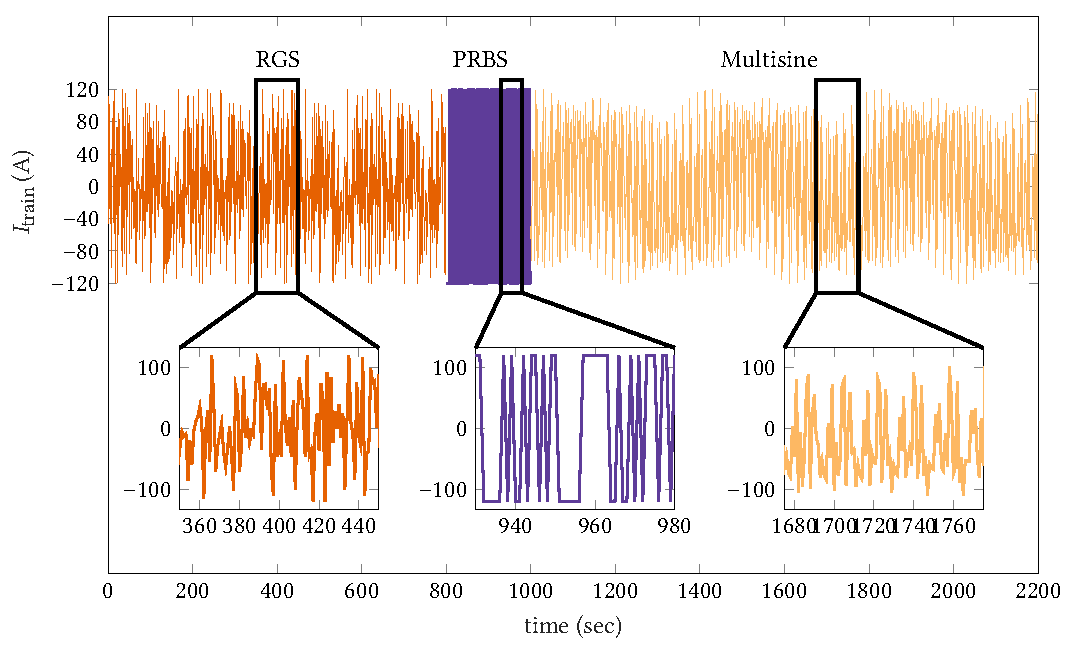
\includegraphics{sysid_validation_input.pdf}
    \captionsetup{singlelinecheck=off}
    \caption[Input current profile used as the validation set for system
    identification]{Input current profile used as the validation set for system
        identification. The sequence consists of
        \begin{enumerate*}[label=\emph{\alph*})]
            \item a \glsfmtlong{rgs},
            \item a \glsfmtlong{prbs}, and
            \item a multisine waveform
        \end{enumerate*}.
        The overall sequence  is intended to emulate the flat  power spectrum of
        white noise (with the \glsfmtshort{prbs}) and excite any poles and zeros
        within  3$\sigma$ spread  of the  \glsfmtshort{rgs} mean.  The multisine
        signal is  swept is composed  of sinusoids with  fundamental frequencies
        from \SI{100}{\milli\hertz}  up to the Nyquist  frequency. Its amplitude
        variation  across the  frequency spectrum  increases the  probability to
        capture the  system's modes that  were possibly missed by  the preceding
        two waveforms.
    }%
    \label{fig:sysidvalidationcurrent}
\end{figure}

\textsc{MATLAB} code  that can be used  to generate the training  and validation
input profiles is shown in \cref{codesnippet:trainvalidsysidinput}.

\begin{listing}[!htbp]
\begin{minted}[mathescape,autogobble,bgcolor=mintedbg,escapeinside=||,texcomments=true]{matlab}
% Needs matlab's system identification toolbox
clear; close all; clc; format short g;
warning('off','Ident:dataprocess:idinput7'); % suppress sysid warnings
I_1C  = 60; % Amps
range = 2*[-I_1C I_1C]; % peak-peak swing is $\pm 2\text{C}=\SI{40}{\ampere}$
NumCh = 1; % no of channels (used by sysid toolbox for multichannel id)
Ts    = 1; % sampling interval

%% Random Binary Input Signal (RBS)
N  = 200; % samples per quantum of each waveform
u1 = idinput(N,'rbs',[],range); % 'idinput' from sysid toolbox
%% Chirp Signal (swept cosine)
t_chirp_start = 0;
t_chirp_end   = 3*N*Ts; %
t             = linspace(t_chirp_start,t_chirp_end,3*N);
f0            = 0;
f1            = 1e-1; % $f_1 = \SI{100}{\milli\hertz}$ is the max chirp frequency
u2            = max(range)*chirp(t,f0,t(end),f1)';
%% Periodic Random Binary Input Signal (Periodic RBS)
bin_seq_Period   = N; % seconds
bin_seq_Period_N = ceil(bin_seq_Period/Ts); % samples
bin_NumPeriod    = 2;
u3 = idinput([bin_seq_Period_N,NumCh,bin_NumPeriod],'rbs',[],range);
%% Random Guassian Signal (RGS)
rgs_Period         = N; % seconds
rgs_Period_samples = ceil(rgs_Period/Ts);
rgs_NumPeriod      = 4;
u4 = idinput([rgs_Period_samples,NumCh,rgs_NumPeriod],'rgs',[],range/2);
%% PseudoRandom Binary Signal (PRBS)
prbs_Period         = N; % seconds
prbs_Period_samples = ceil(prbs_Period/Ts);
u5                  = idinput(N,'prbs',[],range);
%% Multisine signal (sum of sines)
samples_per_Period = 2*N;
NumPeriod          = 3;
[u6,freq] = idinput([samples_per_Period 1 NumPeriod],'sine',[],range);

%% Split into training and validation data sets
I_load_train    = [u1;u2;u3];
I_load_validate = [u4;u5;u6];
\end{minted}
\caption{Generation of training and validation input current profiles in
\textsc{MATLAB}}
\label{codesnippet:trainvalidsysidinput}
\end{listing}


% \section{Investigation of Linearity and Time Invariance}\label{sec:lticheck}
% % -*- root: ../main.tex -*-
%!TEX root = ../main.tex
% this file is called up by main.tex
% content in this file will be fed into the main document
% vim:textwidth=80 fo=cqt


The      transfer     function      identification     techniques      mentioned
in \cref{sec:introblackboxsysid} are  applicable only for \gls{lti}  systems. At
first glance,  this seems to  be overly restrictive  for the system(s)  at hand.
When  considered  as  a  single  macroscopic  entity,  a  lithium  ion  battery,
exhibits  overall non-linear  characteristics,  particularly due  to the  strong
non-linearities in
\begin{enumerate*}[label=\emph{\alph*})]
    \item the Butler-Volmer reaction kinetics (see \cref{eq:butlervolmer}), and
    \item the \glspl{ocp} of the two electrodes (see \cref{eq:lcoUocpPos} and \cref{eq:lcoUocpPos}).
\end{enumerate*}
However,  we are  dealing with  a much  narrower scope  \ie{} the  systems under
consideration  are just  the two  sub-system entities  (one per  electrode) that
transform the  applied current at  a particular  time-step to the  overall moles
per  unit area  of  \ch{Li^+}  ions in  the  corresponding  electrode region  of
the  electrolyte at  that  same  instant. Therefore,  it  is  the linearity  and
time-invariance of these \emph{subsystems} that must be investigated.

\subsection{Time-invariance of the electrolyte time-evolution subsystems}\label{subsec:timeinvariance}
A  test  for time-invariance  is  prescribed  in  the  lecture notes  on  system
identification by  Plett~\cite{PlettECE5560_02}. The steps involved  therein are
reproduced here after  being suitably adapted to the notation  of the subsystems
at hand.
\begin{enumerate}
    \item Apply input $u_1(t) = I(t)$ to the system and measure the outputs $Q_{\text{e,n}_1}\!(t)$ and $Q_{\text{e,p}_1}\!(t)$.
    \item Apply a delayed version of the input by $\tau$ seconds \ie{} $u_2(t) = I(t-\tau)$ to the system and measure the outputs $Q_{\text{e,n}_2}\!(t)$ and $Q_{\text{e,n}_2}\!(t)$.
    \item If $Q_{\text{e,n}_2}\!(t)$ = $Q_{\text{e,n}_1}\!(t-\tau)$ and
        $Q_{\text{e,p}_2}\!(t)$ = $Q_{\text{e,p}_1}\!(t-\tau)$ for all possible
        delays $\tau$, as well as for all choice of input signals $I(t)$, then the systems are time-invariant.
\end{enumerate}

For the systems at hand, it is  not strictly required to apply this prescriptive
test. Unless a fundamental change in the underlying reaction phenomena/chemistry
occur that  alter the  performance over  time, these systems  can be  treated as
time-invariant. Factors  that induce  time-dependent shift  in the  behaviour of
lithium ion batteries are degradation  phenomena such as thickening of \gls{sei}
layer, dendrite growth or mechanical  fatigue in electrodes which in-turn affect
electrolytic  diffusion and  conductivity. Yet  another cause  of time-dependent
behavioural change  is the drift  in parameter values. However,  these phenomena
are  typically  one or  mode  orders  of  magnitude  slower than  the  \gls{p2d}
dynamics\fxnote{citation needed}. This separation  of time-scales imply that, in
practice they can be decoupled. Therefore, separate models can be identified for
the faster and slower processes. A  suitable model-blending approach can then be
considered  to cover  all processes  across time-scales.  Although the  concepts
developed here for the fast electrolyte dynamics can be suitably adapted to such
slow phenomena, their study  falls outside the scope of this  thesis and is left
as an exercise for  future work. Thus, the overall battery  system, and hence by
extension,  the  two subsystems  considered  are  deemed to  be  time-invariant.
However, in the interest of completeness, this author systematically applied the
aforementioned test procedure with every  combination arising from the choice of
ten time-delay values and the following six current profiles ---
\begin{enumerate*}[label=\emph{\alph*})]
    \item constant current 1C discharge,
    \item constant current 3C discharge,
    \item constant current 1C charge,
    \item \gls{udds} input profile with peak amplitude of 3C,
    \item training profile used in system identification (see \cref{fig:sysidtrainingcurrent}), and
    \item validation profile used in system identification (see \cref{fig:sysidvalidationcurrent}).
\end{enumerate*}
Finally,  these tests  were  repeated for  a choice  of  five different  initial
\glspl{soc}   ---   \SI{90}{\percent},   \SI{70}{\percent},   \SI{50}{\percent},
\SI{30}{\percent}  and \SI{10}{\percent}\footnote{\label{fn:socstart}The  number
of  moles  of  \ch{Li^+} per  unit  area  in  the  electrolyte does  not  depend
on  the  electrode's \glsfmtshort{soc}.  However,  different  starting point  of
\glsfmtshort{soc}s were considered  to have a wide variety in  the length of the
recorded  data until  cut-offs  were hit.  \eg{}  starting at  \SI{90}{\percent}
\glsfmtshort{soc} could  mean that  for a  current spike  early in  the profile,
upper  cut-off voltage  shall be  hit  sooner leaving  a smaller  set of  logged
simulation data.}.

\begin{figure}[!htbp]
    \centering
    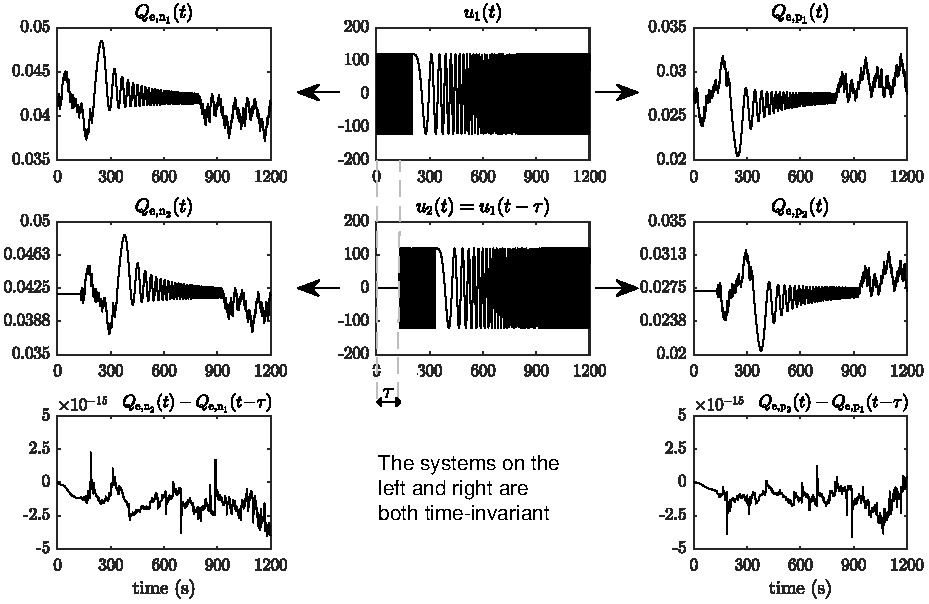
\includegraphics[width=\textwidth]{time_invariance.pdf}
    \caption[Demonstration of time-invariance of $Q_\text{e,n}(t)$ and
    $Q_\text{e,p}(t)$ subsystems]{Demonstration of time-invariance of the
        subsystems considered. The applied current profile $u_1(t)$ is the
        system identification training sequence
        from \cref{fig:sysidtrainingcurrent} (top row of the central column).
        The top left plot shows the response $Q_{\text{e,n}_1}\!(t)$, while that
        on the top right shows $Q_{\text{e,p}_1}\!(t)$. The second row of the
        middle column shows the same input sequence delayed by $\tau =
        \SI{130}{\second}$. Application of this current profile $u_2(t) =
        u_1(t-\tau)$ results in the outputs $Q_{\text{e,n}_2}\!(t)$ and
        $Q_{\text{e,p}_2}\!(t)$ to its left and right respectively. Subtracting
        these from the correspondingly delayed versions of the original outputs
        result in zero residuals, thereby proving time-invariance of these
        subsystems. The jitter shown in the bottom row of plots is
        $\mathcal{O}(10^{-15})$ in magnitude and are due to the numerical
        roundoffs that occur when operating close to the noise floor of the
    machine's floating point units.}%
\label{fig:timeinvariance}
\end{figure}
% The outputs $Q_\text{e,n}$ and $Q_\text{e,p}$ are shown to the left and right of the applied input.

\Cref{fig:timeinvariance}  demonstrates the  time-invariance  of the  subsystems
considered  at  an  initial  \gls{soc} of  \SI{50}{\percent}  for  a  time-delay
of   \SI{130}{\second}   using   the  highly   dynamic   system   identification
training    sequence   that    was   synthesised    by   this    thesis   author
(see \cref{fig:sysidtrainingcurrent}).  The  applied  current  profile  $u_1(t)$
(top row  of the  central column)  produces the  outputs $Q_{\text{e,n}_1}\!(t)$
and  $Q_{\text{e,p}_1}\!(t)$  shown  in  the   top  left  and  top  right  plots
respectively.  When  the delayed  version  of  this  input sequence  ${u_2(t)  =
u_1(t-\tau)}$ (middle row, middle column) is  applied, it results in the outputs
$Q_{\text{e,n}_2}\!(t)$  and  $Q_{\text{e,p}_2}\!(t)$  to  its  left  and  right
respectively.  Following the  steps  of the  test  procedure, subtracting  these
outputs from the correspondingly delayed versions of their original counterparts
result in  zero residuals, thereby  proving time-invariance of  these subsystems
under these representative test conditions. The residual sequences in the bottom
row of plots are of $\mathcal{O}(10^{-15})$ and arise due to numerical roundoffs
that occur  when operating close  to the noise  floor of the  machine's floating
point units.

Similar to  the case demonstrated  here, all  tests for time-invariance  for all
permutations of  the chosen operating  conditions passed successfully  \ie{} the
delayed  version of  the original  output  signals accurately  matched with  the
responses  to  the corresponding  delayed  input  (down to  machine  precision),
thereby confirming the time-variance of  the subsystems considered in the system
identification problem, which enables us to proceed further.


\subsection{Linearity analysis of the electrolyte time-evolution subsystems}\label{subsec:linearityanalysis}

\subsubsection*{De-biasing of  input signals}
In the analyses of linearity of systems, it is a recommended practice to de-bias
the output and input quantities about their mean operating conditions. The input
signal  in this  case is  the applied  load current  $I(t)$, which  can be  both
positive  (during discharge)  and  negative  (during charge).  The  mean of  the
training profile is  \SI{-1.167}{\ampere} and that of the  validation profile is
\SI{-0.3273}{\ampere}. Clearly,  the mean values  are dependent upon  the actual
current profile used. The appropriately de-biased signal \ie{} $\widetilde{I}(t)
= I(t) - \bar{I}(t)$ is to be used  for training and validation data sets in the
system identification procedure. For the purpose  of linearity analysis, it is a
standard practice to simply apply a step change in input (from zero) and measure
the output responses, thereby bypassing the de-biasing requirements.

% Although, in  principle, the strength  of the input  signal does not  affect the
% linearity tests, for  the actual system identification  procedure, the de-biased
% signal must still be persistently exciting as in \cref{sec:persistentexcitation}
% must be

For the output signals, bias  values can be pre-computed analytically and
accounted for.  The overall number  of moles of \ch{Li^+}  per unit area  in any
region within  the cell cannot  be physically  negative. Even though  under high
C-rates,  ion depletion  at localised  spatial  locations (such  as the  current
collectors) is  certainly possible,  the entire thickness  of any  region cannot
become devoid of ions at any point  in time since the cell shall instantaneously
cease  to work.  Thus, for  a typical  well-designed cell  operating within  the
manufacturer prescribed  C-rate limits,  the output signals  under consideration
operate  in  a  small  window  about  their  initial  values.  In  the  author's
simulations, even  at $\pm$5C, the overall  number of moles of  \ch{Li^+} in any
cell region exhibited  a maximum change of less than  \SI{15}{\percent} from its
initial value. Thus,  the de-biased output variables  for system identification,
$\widetilde{Q}_{\text{e,}j}(t)$ can be obtained  by subtracting their respective
initial values $Q_{\text{e,}j}(0)$ (see \cref{eq:Qeninit} and \cref{eq:Qepinit})
from $Q_{\text{e,}j}(t)$.
\begin{align}
    \widetilde{Q}_\text{e,n}(t) & = {Q}_\text{e,n}(t) - {Q}_\text{e,n}(0) \\
    \widetilde{Q}_\text{e,p}(t) & = {Q}_\text{e,p}(t) - {Q}_\text{e,p}(0)
\end{align}
which  implies   that  the   transfer  functions  to   be  identified   have  to
be   modified   to   be   $\frac{\widetilde{Q}_\text{e,n}(s)}{\bar{I}(s)}$   and
$\frac{\widetilde{Q}_\text{e,p}(s)}{\bar{I}(s)}$  respectively.  This  does  not
affect  the  time-invariance  proved in \cref{subsec:timeinvariance}  since  the
initial  values   $Q_{\text{e,}j}(0)$  are   merely  constants  and   hence  not
time-dependent.

\subsubsection*{Test for linearity}
Similar     to      the     test      for     time      invariance     described
in \cref{subsec:timeinvariance}, a  test for linearity is  also prescribed in
the lecture notes on  system identification by Plett~\cite{PlettECE5560_02}. The
steps involved therein  are reproduced here after being suitably  adapted to the
notation of the subsystems at hand. This is essentially a recipe for testing the
superposition principle.
\begin{enumerate}
    \item Apply input profile $I_1(t)$ to the system and obtain outputs $\widetilde{Q}_{\text{e,n}_1}\!(t)$ and $\widetilde{Q}_{\text{e,p}_1}\!(t)$.
    \item Apply a different profile $I_2(t)$ to the system and obtain outputs $\widetilde{Q}_{\text{e,n}_2}\!(t)$ and $\widetilde{Q}_{\text{e,n}_2}\!(t)$.
    \item Now apply an input profile $I_3(t) = \alpha I_1(t) + \beta I_2(t)$ and obtain a corresponding set of outputs $\widetilde{Q}_{\text{e,n}_3}\!(t)$ and $\widetilde{Q}_{\text{e,n}_3}\!(t)$.
    \item If $\widetilde{Q}_{\text{e,n}_3}\!(t)$ = $\alpha\, \widetilde{Q}_{\text{e,n}_1}\!(t) + \beta \, \widetilde{Q}_{\text{e,n}_2}\!(t)$ and $\widetilde{Q}_{\text{e,p}_3}\!(t)$ = $\alpha\, \widetilde{Q}_{\text{e,p}_1}\!(t) + \beta \, \widetilde{Q}_{\text{e,p}_2}\!(t)$ for all possible $\{\alpha,\beta\}$ as well as for choice of input signals $\{I_1(t),I_2(t)\}$, then the systems are linear.
\end{enumerate}

As   in   the  time-invariance   test,   the   same   set  of   five   different
initial  \glspl{soc}\textsuperscript{\ref{fn:socstart}}  ---  \SI{90}{\percent},
\SI{70}{\percent},  \SI{50}{\percent}, \SI{30}{\percent}  and \SI{10}{\percent},
was  retained for  these linearity  tests. For  each test  run, a  pseudo-random
number generator  was used to select  the values of $\{\alpha,\beta\}$  from the
set  of  real numbers  $\mathbb{R}$  (not  restricted  to  the set  of  integers
$\mathbb{Z}$) in  the closed  interval spanning $[-1.25,1.25]$.  Negative values
are acceptable for  both the scaling coefficients since  the resulting composite
input $I_3(t)$ can be either positive or negative. The composite signal $I_3(t)$
was obtained by taking a random combination  of any two of the following current
profiles ---
\begin{enumerate*}[label=\emph{\alph*})]
    \item step input with a constant current 1C discharge,
    \item step input with a constant current discharge at C/5,
    \item step input with a constant current 1C charge,
    \item step input with a constant current charge at C/5,
    % \item de-biased training profile used in system identification (see \cref{fig:sysidtrainingcurrent}), and
    % \item de-biased validation profile used in system identification (see \cref{fig:sysidvalidationcurrent}).
\end{enumerate*}

The  scaling  factors  $\alpha$  and   $\beta$  were  restricted  to  the  range
$[-1.25,1.25]$ in consideration of limiting the peak applied current to within a
\pm 3C  window ---  the operating  condition for most  \glspl{bev}, so  that the
isothermal assumption for the model shall remain valid. This peak current corner
case occurs when the pseudo-random generator chooses both scaling factors at the
selected range's limits for the 1C constant current discharge or charging cases.
The limited  range of the  scaling factors are also  motivated by the  fact that
most real-world systems remain linear only within a certain operating window. In
particular, care  must be taken to  ensure that the cell's  \gls{soc} during the
linearity test  remains within  its physical limits  for any  initial \gls{soc}.
Furthermore, localised  saturation or depletion  of ions for  extended durations
must be avoided. Hence  it can be concluded that, with the  chosen range for the
scaling  factors,  if  the  two subsystems  under  consideration  remain  linear
everywhere below  a peak  current of  \pm 3C  in the  isothermal case,  then the
linearity  tests are  considered as  passed.  Future extensions  to undertake  a
temperature-dependent  system  identification  exercise can  potentially  use  a
first-order Taylor  expansion about this  operating window. The  discussion thus
far  has fully  established  all  the conditions  for  conducting  the test  for
linearity.

\begin{figure}[!htbp]
    \centering
    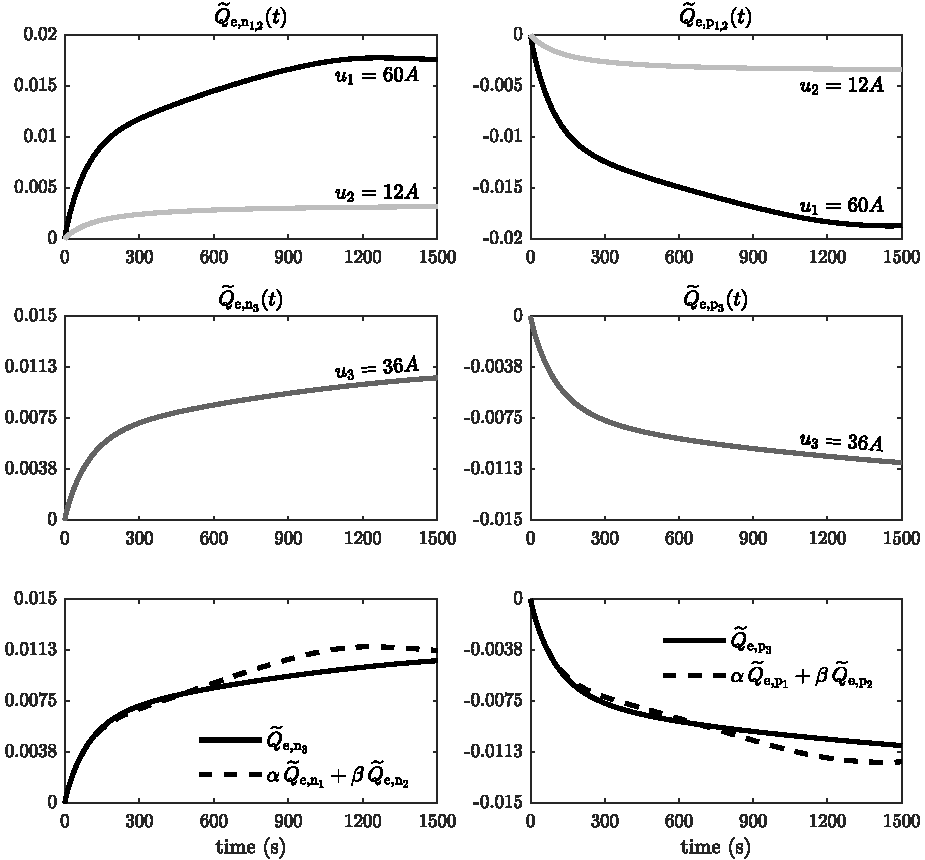
\includegraphics[width=\textwidth]{linearity_proof}
    \caption[Illustration of linearity test for the
    \protect{$\widetilde{Q}_{\text{e,n}}$} and
    \protect{$\widetilde{Q}_{\text{e,p}}$} subsystems]{Illustration of one
        instance of linearity tests for the subsystems under consideration. For
        this visualisation, constant current inputs are used throughout. The top
        row of plots shows $\widetilde{Q}_{\text{e,n}}$ and
        $\widetilde{Q}_{\text{e,p}}$ for two step inputs $I_1(t) =
        \SI{60}{\ampere}$ and $I_2(t) = \SI{12}{\ampere}$ \ie{} discharge with
        1C and C/5 currents respectively. The second row of plots shows
        $\widetilde{Q}_{\text{e,n}_3}$ and $\widetilde{Q}_{\text{e,p}_3}$  for
        $I_3 = \SI{36}{\ampere}$, where $I_3 = \alpha I_1 + \beta I_2$ with
        $(\alpha,\beta) = (1,-2)$. The last row of plots overlays these
        quantities with the manually computed linear combination of their two
        preceding responses. Had these sequences overlapped exactly, the systems
        would have been exactly linear. Despite exhibiting deviations over the
        considered horizon, the transient responses in both electrode regions do
        follow the superposition principle. Even past the transient, maximum
        error in both cases is an order of magnitude lower than the individual
        outputs. Hence, the two systems are deemed to be \emph{approximately}
        linear.
    }%
    \label{fig:linearity}
\end{figure}

\Cref{fig:linearity}  illustrates  one  instance  of a  linearity  test  wherein
constant  currents  and  integer  scaling  factors are  used  for  the  sake  of
illustration.  The  plots   in  the  left  column  deal   with  the  electrolyte
time-evolution  subsystem  in  the  negative electrode  region.  Similarly,  the
plots  in  the  right  column  deal with  the  corresponding  subsystem  in  the
positive electrode region.  A discharge current of 1C  \ie{} \SI{60}{\ampere} is
first  applied  and  the  corresponding  outputs  $\widetilde{Q}_{\text{e,n}_1}$
and   $\widetilde{Q}_{\text{e,p}_1}$  are   obtained.   Secondly,  a   discharge
current   of   C/5   \ie{}   is    applied   and   the   corresponding   outputs
$\widetilde{Q}_{\text{e,n}_2}$ and  $\widetilde{Q}_{\text{e,p}_2}$ are obtained.
These set of responses are plotted  in the top row of \cref{fig:linearity}. Now,
a  third  value  of  input  current $I_3$,  computed  as  a  linear  combination
of  the  previous  input  currents  \ie{}  $I_3 =  \alpha  I_1  +  \beta  I_2  $
is  applied.  For  illustrative  purposes, the  integer  set  $(\alpha,\beta)  =
(1,-2)$  was  chosen  for  the   scaling  coefficients,  which  implies  $I_3  =
\SI{12}{\ampere}$. The corresponding  outputs $\widetilde{Q}_{\text{e,n}_3}$ and
$\widetilde{Q}_{\text{e,p}_3}$ are  plotted in the  middle row. As per  the test
for linearity,  if these signals are  equal to the signal  generated by manually
computing the linear  combination of the preceding two outputs,  then the system
is linear.

The   plots   in  the   third   row   show  $\widetilde{Q}_{\text{e,n}_3}$   and
$\widetilde{Q}_{\text{e,p}_3}$ overlaid with their respective linear combination
signals. In  the case  of the  subsystem in the  negative electrode  region, the
transient performance matches  precisely until \approx\SI{450}{\second}, whereas
that in the positive electrode region exhibits a good matching for approximately
the  first  \SI{250}{\second}.  However,  for the  horizon  considered  the  two
overlaid plots do not overlap exactly.  Hence, the systems are not truly linear.
However, the exhibited  behaviour is quite close to linearity,  with the maximum
absolute  error  in each  region,  even  outside  the initial  transient,  being
$\mathcal{O}(10^{-4})$  --- an  order  of magnitude  lower  than its  individual
components.  This behaviour  was exhibited  for all  test instances  considered.
Considering  that for  dynamic  simulation runs,  the  transient performance  is
paramount  to  the good  performance  of  the  model,  in conjunction  with  the
aforementioned  low error  metric,  these  subsystems can  be  considered to  be
\emph{approximately} linear.

Based  on  the  analysis  presented   here,  \gls{lti}  behaviour  for  the  two
subsystems is  assumed, which facilitates  in proceeding with the  actual system
identification procedure.




% \section[Transfer Function Identification Procedure]{Transfer Function Identification Procedure\footnote{The early stages of this section presents this author's digested summary of the theoretical framework adapted from a subset of content from the lecture notes on system identification by Plett~\cite{PlettECE5560_02,PlettECE5560_03,PlettECE5560_04}.}}\label{sec:actualsysid}
% % -*- root: ../main.tex -*-
%!TEX root = ../main.tex
% this file is called up by main.tex
% content in this file will be fed into the main document
% vim:textwidth=80 fo=cqt

\subsection{The transfer operator and its model form}
In a classical system identification  task, the discrete-time transfer functions
for the systems  under consideration need to be  determined. These discrete-time
transfer functions are  based on Z-transforms in the  frequency domain. However,
for the purpose of working in time-domain, an analogous linear operator $q$ that
performs a  forward shift on  its input \ie{} $  {q u[k] \longmapsto  u[k+1]} $.
Similarly, applying the  backward shift operator $ q^{-1} $  on the input yields
its value at the previous time-step \ie{} $ {q^{-1} u[k] \longmapsto u[k-1]}$.

\begin{figure}[!htbp]
    \centering
    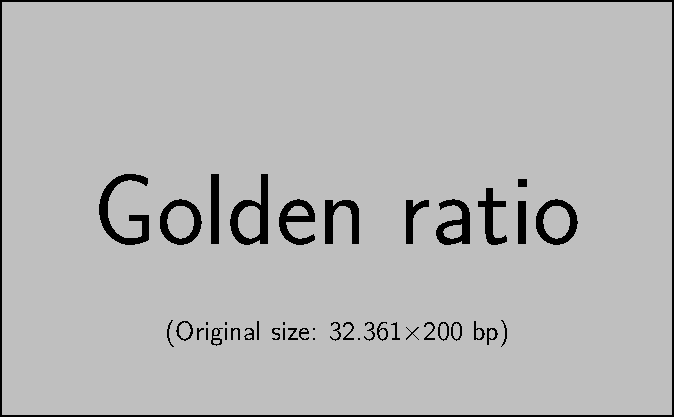
\includegraphics{placeholder_images/example-image-golden.pdf}
    \caption[Block diagram representing a generic discrete-time \glsfmtshort{lti} system]{%
        Block  diagram representing  a  generic discrete-time  \glsfmtshort{lti}
        system. The  control input $u[k]$ is  acted upon by the  system dynamics
        $G[k]$  whereas a  white  noise  input $e[k]$  is  shaped  by the  noise
        dynamics $H[k]$. The  overall output $y[k]$ consists  of a superposition
        of the contribution from both these components.
    }%
    \label{fig:genericltisyswithnoise}
\end{figure}

\Cref{fig:genericltisyswithnoise} shows  a generic \gls{lti} system  wherein the
measurements are corrupted by noise. The  system dynamics are represented by the
transfer operator $G(q)$\footnote{The term transfer  operator in the time domain
mathematically  corresponds  to the  term  transfer  function in  the  frequency
domain.  Mathematically,  $G(q) =  G(z)\bigr\rvert_{\mathrlap{z=q}}$.}  that  acts on  the
applied  input  $u[k]$,  whereas  the  noise dynamics  are  represented  by  the
disturbance operator  $H(q)$ that  acts to  filter (or  shape) an  assumed white
noise input $e[k]$.

Assuming linearity and time-invariance throughout, the overall output can be
written as the linear combination
\begin{equation}\label{eq:outputwithsysandnoise}
    % \SwapAboveDisplaySkip
    y[k] = G(q)u[k] + H(q)e[k]
\end{equation}
where $G(q) = \frac{B(q)}{A(q)}$ and $H(q) = \frac{C(q)}{D(q)}$ are the transfer
operators describing the dynamics of the system and disturbance respectively.

$A(q), B(q), C(q)$ and $D(q)$ are rational polynomials in $q$. The two transfer
operators $G(q)$ and $H(q)$ can be represented by
\begin{align}
    G(q) &= q^{-n_k}\frac{b_1q^{-1} + \dots  + b_{n_b}q^{-{n_b}}}{1 + a_1q^{-1} + \dots  + a_{n_a}q^{-{n_a}}} \\
    H(q) &= q^{-n_l}\frac{c_1q^{-1} + \dots  + c_{n_c}q^{-{n_c}}}{1 + d_1q^{-1} + \dots  + d_{n_d}q^{-{n_d}}}
\end{align}
where $(n_k,n_l)$ represent  the number of transport  delay samples, $(n_b,n_c)$
the number  of feedforward coefficients  and $(n_a,n_d)$ the number  of feedback
coefficients in $G(q)$ and $H(q)$ respectively.


In  this  system  identification  task  at hand,  the  output  measurements  are
collected from a  \emph{noise-free} simulation of the \gls{p2d}  model \ie{} the
disturbance transfer operator in~\cref{eq:outputwithsysandnoise} is zero
\begin{align}
    y[k] &= G(q)u[k] + \cancelto{0}{H(q)}e[k]
\shortintertext{Hence, the time-domain output  reduces  to}
y[k] &= G(q)u[k] \label{eq:outputwithsysonly}
\end{align}

Thus, the system identification task becomes one that of estimating
\begin{enumerate}
    \item The number of transport delay samples $n_k$.
    \item The number of feedforward coefficients (zeros) $n_b$.
    \item The zeros themselves $b_1, b_2, \dots b_{n_b}$.
    \item The number of feedback coefficients (poles) $n_a$.
    \item The pole locations $a_1, a_2 \dots a_{n_a}$.
\end{enumerate}
for  each  of  the  two  transfer operators  $G_1(q)$  and  $G_2(q)$  \ie{}  the
electrolyte  time-evolution subsystems  in the  negative and  positive electrode
region respectively.

\subsection{Estimation of transport delay}

The transport delay $n_k$ can be estimated visually by inspecting the step
response of the systems under consideration.

In~\cref{fig:linearity},   step  inputs   of   $I_1   =  \SI{60}{\ampere},   I_2
=    \SI{12}{\ampere},$   and    $I_3   =    \SI{36}{\ampere}$   were    applied
to    the   two    subsystems.    Inspecting   closely    all   the    responses
\ie{}   $\widetilde{Q}_{\text{e,n}_1},    \widetilde{Q}_{\text{e,n}_2}   $   and
$\widetilde{Q}_{\text{e,n}_3}$    in    the     negative    electrode    region,
and    $\widetilde{Q}_{\text{e,p}_1},    \widetilde{Q}_{\text{e,p}_2}   $    and
$\widetilde{Q}_{\text{e,p}_3}$  in the  positive electrode  region, it  is clear
that all these outputs start exactly at  zero. Therefore, there is no delay term
to be considered for the transfer operators \ie{} $n_k = 0$ for both subsystems.

\subsection{Choice of model structure}\label{subsec:modelstrucchoice}

Among      the      transfer-function       model      structures      mentioned
in~\cref{subsec:parametric}, the \gls{arx} model  structure is too simplistic to
consider. Despite  the fact that  its numerical computation involves  only basic
linear algebra operations,  that can be efficiently handled  on modern computing
systems, it  is considered to produce  poor estimates of the  system's poles and
zeros. In the absence of contributions from the noise-term, the all-encompassing
model structure used by the Box-Jenkins approach is deemed to be unnecessary for
the  problem  at hand.  Therefore,  the  two  model structures  considered  were
\gls{armax} and \gls{oe} for the coefficient determination.

\subsection{Starting guesses for coefficient orders}\label{subsec:initguesscoefforder}

At first, the training profile of~\cref{fig:sysidtrainingcurrent} is
debiased (through mean removal) and applied as the input current profile in a \gls{p2d}
simulation. The outputs of this simulation are suitably post-processed as per
the following sequence of steps.
\begin{enumerate}
    \item The concentrations solved at various node locations within each
        electrode are numerically integrated over the corresponding electrode
        thicknesses using trapezoidal rule.
    \item The resulting integral value is multiplied with the porosity of the
        corresponding electrode region to obtain $Q_{\text{e,n}_\text{train}}(t)$ and
        $Q_{\text{e,p}_\text{train}}(t)$.
    \item These quantities are then de-biased by subtracting their initial
        values to obtain $\widetilde{Q}_{\text{e,n}_\text{train}}(t)$ and
        $\widetilde{Q}_{\text{e,p}_\text{train}}(t)$.
\end{enumerate}

The        same        procedure        is        repeated        for        the
validation       current      profile       of~\cref{fig:sysidvalidationcurrent}
to         obtain         $\widetilde{Q}_{\text{e,n}_\text{val}}(t)$         and
$\widetilde{Q}_{\text{e,n}_\text{val}}(t)$.  These data  sets are  used for  all
subsequent sub-tasks involved in this system identification exercise.

In  order to  reduce  the search  window for  the  coefficient determination  in
the  parametric transfer  function methods,  the hand-estimation  of coefficient
order  through non-parametric  methods may  be performed.  This coarse  estimate
can  act as  a  feeder to  help  in  the faster  convergence  of the  non-linear
optimisation algorithms  used in the parametric  methods. In this case,  a basic
spectral analysis  using a Hanning  window implemented using the  MATLAB command
\texttt{spa.m} is applied to the time-domain data to transform it into frequency
response data.

\begin{figure}[!htbp]
    \centering
    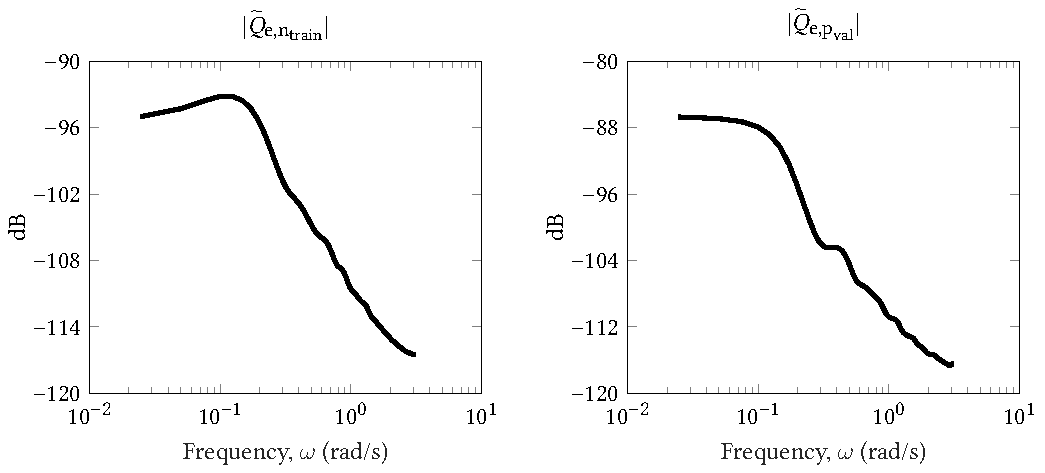
\includegraphics[width=\textwidth]{bode_mag.pdf}
    \caption[Bode magnitude plots of the electrolyte time-evolution sub-systems]{%
        Bode magnitude  plots showing the  estimated frequency response  for the
        two  subsystems under  consideration.  The frequency  response data  was
        obtained  through a spectral  analysis \ie{}  by computing  the ratios  of
        spectra of the de-biased input  and output sequences. The sequences were
        smoothed using a Hanning window before computing the ratio.
    }%
    \label{fig:initialbodemag}
\end{figure}

\Cref{fig:initialbodemag}  shows  the  Bode  magnitude  plot  of  the  frequency
response for
\begin{enumerate*}[label=\emph{\alph*})]
    \item the training set in the negative electrode region, and
    \item the validation set in the positive electrode region.
\end{enumerate*}
In the  plots, a broad  combination of  the two data  sets in the  two electrode
region  is  depicted  to  achieve  a  compact  representation  of  all  possible
permutations and to avoid redundancies by plotting visually similar information.
It is important to note that these Bode diagrams obtained by such non-parametric
methods only represent  a crude approximation of the  physical dynamics intended
to help in initial estimates of the system behaviour.

Some preliminary understanding of the  various characteristics of the system can
be gleaned from these Bode diagrams.  The first visually striking feature is the
similarity  in the  approximate frequency  characteristics in  the negative  and
positive electrode  regions, even when  excited by completely different  data in
the time domain. This confirms the author's assumptions of equal `complexity' in
the symbolic  regression search discussed in~\cref{subsec:symbolicreg}.  This is
also  congruent with  the physical  behaviour of  the electrolyte  in these  two
regions.

\subsubsection*{Finite DC gain}
By visual  extension of  the frequency responses  towards lower  frequencies, it
is  clear  that  the  DC  gains  of  both  the  systems  are  finite  and  below
unity.  This  behaviour  can  clearly  be  seen  in  the  time-domain  responses
of~\cref{fig:linearity}.  For  the plotted  time-horizon,  this  effect is  most
visible for the case of the \SI{12}{\ampere} constant current input, wherein the
responses of both regions settle to a finite value after an initial transient.

There is \approx\SI{10}{\decibel} variability in  the low frequency gain between
the two Bode  plots in~\cref{fig:initialbodemag}. This can be  attributed to the
following  factors. A  compromise with  the spectral  estimation method  is that
using a higher number of frequency bins  results in lower resolution per bin and
vice-versa. By  varying the number  of frequency bins  and focussing on  the low
frequency range, the resolution of the DC  gain can be improved. The rest of the
variability can  be attributed to the  fact that the training  and test profiles
behave differently and do not excite the same dynamics. In particular, the swept
frequency cosine (chirp) signal in the training set was specifically designed to
draw out  the low frequency  dynamics with a  high fidelity. Finally,  the small
range of variation in the DC gain could also be due to the intrinsic small-scale
variations of  the electrolyte  behaviour in  these two  regions. Although  on a
macroscopic frequency scale the two regions behave similarly, the differences in
electrode thicknesses and porosities could contribute to the small difference in
the  DC gain.  This  helps  to confirm  that  two \emph{non-identical}  transfer
functions are being sought for --- one for each electrode region.

Finally, the finiteness  of the DC gain  helps to narrow down  the search window
for the parametric model structures. In particular, this fact indicates that the
model structures to be trialled must not  have any integrator terms (or poles at
the origin of the complex plane).

\subsubsection*{Resonance and model order}

First  order  transfer   functions  do  not  exhibit   characteristic  peaks  or
resonances  in  their  frequency  responses.  However,  for  the  Bode  plot  on
the   left   of~\cref{fig:initialbodemag},   a   pronounced   resonance   around
\SI{0.15}{\radian\per\second} is observable. This has  an enormous impact --- it
presents  an important  clue  that the  first  order time-evolution  \glspl{ode}
of~\cref{eq:negliionmolesquadratic}   and~\cref{eq:posliionmolesquadratic}   are
inadequate to represent the system dynamics.

An apparent  contradiction to  the first-order inadequacy  claim stems  from the
Bode plot  on the  right hand side  in~\cref{fig:initialbodemag}. In  this case,
there are no resonances in the  magnitude response indicating that a first order
model description is sufficient. However, a vital aspect to be noted here is the
nature of the  validation current profile when compared to  that of the training
current profile.  The coarse  frequency response data  obtained by  the spectral
method is sensitive to the actual  input sequence employed. From systems theory,
the  resonances at  a frequency  occur  due to  the presence  of lightly  damped
complex conjugate poles at that frequency. The periodic \gls{rgs} was explicitly
designed in the  training set and is  however absent in the  validation set. The
unique characteristics  of the validation  set and its influence  on coefficient
order is discussed next.

As per  the arguments presented  in the  preceding discussions, there  exists an
implicit constraint that  the behaviour of the time-evolution  subsystems in the
two electrode  regions are  expected to be  of similar  `complexity'. Therefore,
based  on the  presence of  the resonance  in the  Bode magnitude  plot for  the
response to  training profile  in the  negative electrode region,  it has  to be
concluded that the two subsystems are \emph{at-least} of second order.

\subsubsection*{Estimation of number of poles and zeros}

The  high-frequency  roll-off  in  the   slopes  of  the  Bode  magnitude  plots
in~\cref{fig:initialbodemag} provide clues on the number of poles in the system.
The  corner  frequency $\omega_\text{c}$  in  both  cases  appear to  be  around
\SI{0.15}{\radian\per\second}.  The  high-frequency  slope of  both  systems  is
\approx\SI{20}{\decibel} per decade,  which implies that they  have at-least one
more pole than the number of zeros if using a continuous time transfer function.
For the  corresponding z-domain  transfer function, this  implies that  $n_a \ge
n_b$.

In the  aspect of estimating the  number and locations of  zeros, the validation
profile outshines  the training profile. While  the Bode plot obtained  with the
training profile  does not indicate  the presence of  zeros in the  systems, the
plateau in \SIrange{0.3}{0.4}{\hertz} range for  the Bode plot of the validation
profile clearly contradicts this. Once again, hypothesising that the two systems
(in the two electrode regions)  have fundamentally identical behaviour with only
small differences owing  to differences in their parameter  values, there exists
at-least one zero in these  continuous-time systems around this frequency range.
The discrete-time discretisation process adds an additional zero to the system.

Based on this preliminary  analysis, the estimates are $n_k = 0,  n_b \ge 2, n_a
\ge 3$.  Only asymptotic approximations  to corner frequencies can  be estimated
from the  Bode plots. Furthermore, the  estimated locations are not  used in the
parametric system identification algorithms and  is of much less importance than
the  model order  estimates.  With this  initial  understanding, the  parametric
system identification procedure is carried out.

\subsection{Refinement of coefficient orders using deterministic criteria}\label{subsec:refinementofcoefforder}

The initial estimate  of coefficient orders in~\cref{subsec:initguesscoefforder}
was performed  based only on  a visual inspection  of the Bode  magnitude plots.
Owing to  the fact that  the frequency  response data is  the result of  a crude
ratio of  spectra, there is a  high probability of missing  vital information on
the number and locations of poles and zeros. Hence only a lower bound on the
coefficient orders are available until this point. Next, a set of deterministic
criteria is used to widen and refine the coefficient order range.


Although   the   \gls{arx}   structure   is  deemed   to   be   too   simplistic
(see~\cref{subsec:modelstrucchoice}), owing to the fact that only linear algebra
operations are involved, as opposed  to numerical optimisation routines employed
in the  \gls{oe}, \gls{armax} and Box-Jenkins  structures, certain deterministic
criteria for  coefficient order  selection can  be incorporated  for coefficient
order selection.
This  can serve  as  a  refinement  of  the
initial number of  coefficients guessed from the Bode  magnitude plots discussed
in.

For any model structure used, its error can be defined as
\begin{align}
    % \SwapAboveDisplaySkip
    \varepsilon[k]      & = y[k] - \hat{y}_\text{m}[k] \label{eq:sysiderroronlyk}\\
    \shortintertext{where $y[k]$ are true measurements and}
    \hat{y}_\text{m}[k] & = G(q)u[k] \tag{\cref{eq:outputwithsysonly} revisited}
\end{align}
are the model outputs obtained by the assumed transfer operator $G(q)$ (which is
to be determined).

The  number of  numerator  and denominator  coefficients in  $G(q)$  as well  as
their  values are  to  be determined.  This  set of  unknowns  can be  collected
into a  parameter vector  $\theta$. Thus, as  per~\cref{eq:sysiderroronlyk}, the
error  sequence is  parametrised by  $\theta$, and  its notation  is amended  to
$\varepsilon[k;\theta]$.

For  an  input-output  data  set  consisting of  $N$  samples,  a  generic  cost
function that may  be applied for all the four  model structures \viz{\gls{arx},
\gls{armax}, \gls{oe} and Box-Jenkins} is
\begin{align}
    V_N(\theta)  & = \sum_{k=1}^N L\left(\varepsilon\left[k;\theta\right]\right)
\shortintertext{where $L(\cdot)$ is a postive-valued scalar loss function.}
\intertext{In a typical system identification task, the sum of squares of the error sequence is  used as the typical loss function, thereby yielding}
    V_N(\theta)  & = \sum_{k=1}^N \varepsilon^2[k;\theta]\label{eq:nonlincostfcnsysid}
    \shortintertext{The vector $\hat{\theta}$ that minimises this cost function is desired}
    \hat{\theta} & = \text{arg}\,\underset{\theta}{\text{min}} V_N(\theta)
\end{align}

For  the \gls{arx}  model structure,~\cref{eq:nonlincostfcnsysid}  reduces to  a
standard quadratic optimisation  problem which may be  solved analytically using
least  squares  linear  algebra.  However,  for  robustness  against  estimation
bias,  instead of  the  standard \gls{ols}  estimates,  the \gls{iv}  estimation
method~\cite{Ljung1999} was used  for this model order  selection task. Applying
this to  the \gls{arx} model  structure, two deterministic model  order criteria
have been defined ---
\begin{enumerate*}[label=\emph{\alph*})]
    \item \gls{aic}, and
    \item \gls{mdl}~\cite{Ljung1999}.
\end{enumerate*}

In  the \gls{aic},  the  optimal  number of  parameters,  $\hat{d}$ in  $\theta$
is  obtained   by  minimising   the  modified   log  likelihood   cost  function
\begin{equation}
    V_{N,\text{mod}}(\theta) =  \ln V_N(\theta)  + \frac{2  d}{N}, \quad N \gg d
\end{equation}
In the \gls{mdl} criterion, this cost function is modified to
\begin{equation}
    V_{N,\text{mod}}(\theta) =  V_N(\theta)\left(1 + \frac{d\, \ln N}{N}  \right)
\end{equation}

For the two subsystems at hand, both  criteria converged to the same choices for
the coefficient orders,  yielding $n_a = 4,  n_b = 4$ and $n_k  = 0$. Therefore,
these values  were used as the  starting points for the  non-linear optimisation
algorithms  used in  determining  the  exact pole  and  zero  locations for  the
discrete-time transfer functions which is described next.

\subsection{Final transfer function coefficients --- Nonlinear optimisation}

For         the         \gls{armax}        and         Box-Jenkins         model
structures,~\cref{eq:nonlincostfcnsysid} results  in a non-linear  cost function
which  is  minimised iteratively  using  quasi-Newton  approaches. The  theoretical
foundation  of  standard non-linear  optimisation  methods  such as  L-BFGS  and
Levenberg-Marquardt are  well established whose  detailed explanation is  out of
the scope of this thesis. Although state of the art methods are not covered, the
interested reader  may consult the  textbook by Scales~\cite{Scales1985}  for an
introductory overview of this topic.

The  final  model structures  (for  both  the  positive electrode  and  negative
electrode time-evolution subsystems) in the z-domain are given by
\begin{equation}
    G(z) = \frac{b_1z^{-1} + \dots + b_{n_b}z^{-{n_b}}}{1 + a_1z^{-1} + \dots + a_{n_a}z^{-{n_a}}}\label{eq:genericZtf}
\end{equation}
wherein the coefficients in the numerator and denominator are to be determined.

The  number of  coefficients obtained  from~\cref{subsec:refinementofcoefforder}
was  used as  the initial  guess for  the coefficient  orders in  the non-linear
optimisation.  For  the  initial  guesses   for  the  numerical  values  of  the
coefficients $(a_1, a_2,  \dots a_{n_a})$ and $(b_1, b_2, \dots  , b_{n_b} )$, a
randomised  multi-start  algorithm was  used.  For  the two  transfer  functions
identified, no distinction is made  between whether the \gls{armax} structure or
Box-Jenkins structure was  used to arrive at the coefficients.  Since the output
magnitudes of $\widetilde{Q}_{\text{e,n}}$  and $\widetilde{Q}_{\text{e,p}}$ are
of  $\mathcal{O}{10^{-3}}$,  a  constant  scaling   factor  of  $k  =  1000$  is
used  to  bring the  order  of  magnitude of  output  data  values to  unity.  A
well-chosen  scaling factor  is often  vital  to the  convergence of  non-linear
optimisation algorithms.  Since the system  is linear, this constant  gain shall
not fundamentally change the dynamics of the  system and can be accounted for by
using the reciprocal  scaling factor of 0.001 in  numerical implementations. The
identification procedure  was carried  out using MATLAB's  System Identification
Toolbox~\cite{matlabsysidtool}.

% -*- root: ../main.tex -*-
%!TEX root = ../main.tex

% \begin{table}[!htb]
%     \centering
%     \caption{}
%     \label{}
%     \begin{tabular}{@{} c | c S[table-format=3.2] c c | c c c c}\toprule
%         Order            & $b_0$    & $b_1$     & $b_2$    & $b_3$     & $a_1$  & $a_2$  & $a_3$  & $a_4$  \\ \midrule
%         \engordnumber{2} & 0.002589 & -0.002472 & {}       & {}        & -1.922 & 0.9227 & {}     & {}     \\
%         \engordnumber{4} & 0.002842 & -0.00753  & 0.006595 & -0.001906 & -3.577 & 4.767  & -2.801 & 0.6118 \\
%         \bottomrule
%     \end{tabular}
% \end{table}

\begin{table}[!htb]
    \centering
    \caption{}
    \label{}
    \begin{tabular}{@{}lS[table-format=3.2] S[table-format=3.2]@{}}
        \toprule
        Foo & \textbf{Normal} & \textbf{Bold} \\
        \midrule
        foo1 & 111 & 111 \\
        foo2 & 222.2 & 222.2 \\
        foo3 & 3.33 & 3.33 \\
        foo4 & 4 & 4 \\
        foo5 & 5.5 & 5.5 \\
        \bottomrule
    \end{tabular}
\end{table}


\Cref{tbl:sysidnegcases}   shows   the   results  obtained   by   applying   the
aforementioned   non-linear  identification   routines  to   the  time-evolution
subsystems in the negative electrode region. The coefficient orders tried in the
system identification  procedure were informed  by the inferences from  the bode
magnitude plots as well as that obtained by applying the deterministic \gls{aic}
and \gls{mdl}  criteria. Only those  models that yielded similar  errors (within
\SI{0.5}{\percent}) across both input datasets were retained.

As  discussed  in~\cref{subsec:initguesscoefforder},   a  first  order  transfer
function cannot capture all the  dynamics of the subsystems under consideration.
Therefore, the lowest order tried in  the identification procedure was two (case
A in~\cref{tbl:sysidnegcases}).  As higher order  models were tried,  the system
accuracy improves steadily as  seen in cases B and C. However  in order to avoid
overfitting, the  \emph{lowest} order  model that  produces the  highest matched
accuracy across both training and validation profiles must be chosen.

Case D illustrates  the importance of the initial values  used in the non-linear
optimisation algorithms.  Despite using an  identical number of  coefficients as
case C,  the optimisation algorithm  converges to  a radically different  set of
zeros  and  poles  resulting  in  a  percentage  error  comparable  to  that  of
the  simple second  order  case. The  fourth  order model  from  case C  (shaded
grey  in~\cref{tbl:sysidnegcases}) performs  the best  across both  training and
validation profiles and  is chosen as the final model.  The number of numerators
and  denominators match  exactly that  predicted by  the deterministic  criteria
given in~\cref{subsec:refinementofcoefforder}. A similar selection procedure was
applied  for  the  identification  of the  transfer  function  corresponding  to
$\widetilde{Q}_{\text{e,p}}$ in the positive electrode region.

The final identified transfer functions (for the scaled output) are
\begin{align}
    \frac{\widetilde{Q}_{\text{e,n}}(z)}{\widetilde{I}(z)} & = \frac{0.002842 z^{-1} - 0.00753 z^{-2} + 0.006595 z^{-3} - 0.001906 z^{-4}}{1 - 3.577 z^{-1} + 4.767 z^{-2} - 2.801 z^{-3} + 0.6118 z^{-4}} \label{eq:finaldisctfneg}\\
    \frac{\widetilde{Q}_{\text{e,p}}(z)}{\widetilde{I}(z)} & = \frac{-0.002809 z^{-1} + 0.007139 z^{-2} - 0.005944 z^{-3} + 0.001614 z^{-4}}{1 - 3.464 z^{-1} + 4.444 z^{-2} - 2.495 z^{-3} + 0.515 z^{-4}}\label{eq:finaldisctfpos}
\end{align}

\begin{figure}[!htbp]
    \centering
    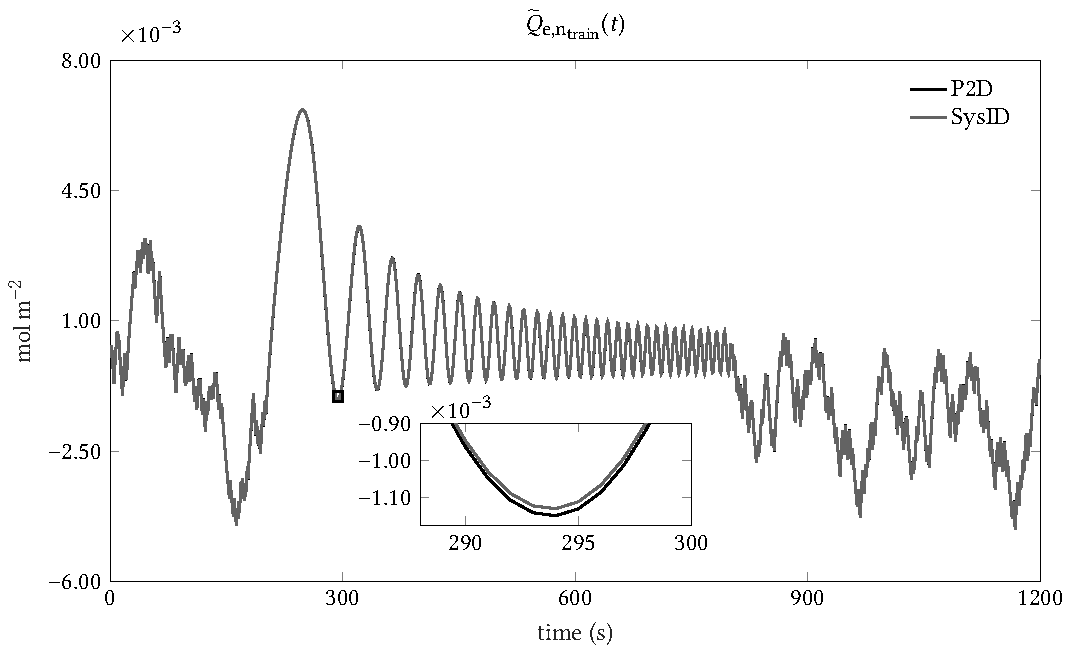
\includegraphics{p2d_sysid_train_qen.pdf}
    \caption[$\widetilde{Q}_{\text{e,n}}(t)$ outputs from \glsfmtshort{p2d} and
    identified transfer function for training profile]{%
        Time-evolution of $\widetilde{Q}_{\text{e,n}}$ computed using the
        \glsfmtshort{p2d} model  and the identified transfer function
        of~\cref{eq:finaldisctfneg} (scaled by 0.001) with the synthetic
        training input profile of~\cref{fig:sysidtrainingcurrent}. The output
        predicted by the identified transfer function closely matches the `true'
        output obtained by a high-fidelity \glsfmtshort{p2d} simulation with an
        \glsfmtshort{rms} error of \SI{5.70e-6}{\mole\per\meter\squared} and a
        \glsfmtshort{mae} of \SI{19.19e-6}{\mole\per\meter\squared}. Note that the
        transfer function in~\cref{eq:finaldisctfneg} was originally obtained by
        scaling the output by 1000. The transfer function output is
        multiplied by the reciprocal of the same scaling factor to obtain the
        predicted response shown here, thereby once again justifying the
        linearity assumption for this subsystem.
    }%
    \label{fig:tfpredQentrain}
\end{figure}

\Cref{fig:tfpredQentrain} shows a comparison of the $\widetilde{Q}_{\text{e,n}}$
output for
\begin{enumerate*}[label=\emph{\alph*})]
    \item the \gls{p2d} model, and
    \item the identified transfer function of~\cref{eq:finaldisctfneg}
\end{enumerate*}
using  the  training  current  profile  of~\cref{fig:sysidtrainingcurrent}.  The
transfer function of~\cref{eq:finaldisctfneg} was obtained by scaling the output
of the  training profile to  be of order $\mathcal{O}(1)$  by a factor  of 1000.
Therefore,  for final  implementation and  comparison purposes,  the raw  output
produced  by applying  the transfer  function  needs to  be scaled  back by  its
reciprocal. If  the system  is linear,  then this scaling  factor shall  have no
impact  on  the  frequency-dependent  dynamics  of  the  subsystem.  The  output
predicted  by the  identified transfer  function is  virtually indistinguishable
from  the `true'  output computed  by post-processing  the \gls{p2d}  model with
an  \glsfmtshort{rms}  error   of  \SI{5.70e-6}{\mole\per\meter\squared}  and  a
\glsfmtshort{mae} of \SI{19.19e-6}{\mole\per\meter\squared}.  This high accuracy
of the transfer  function prediction justifies the linearity  assumption for the
subsystem.  \Cref{fig:tfpredQepval}  presents  the  same  comparison  using  the
validation input profile for the subsystem in the positive electrode region. The
accuracy of  the identified transfer function  for this independent data  set is
clearly illustrated.

\begin{figure}[!htbp]
    \centering
    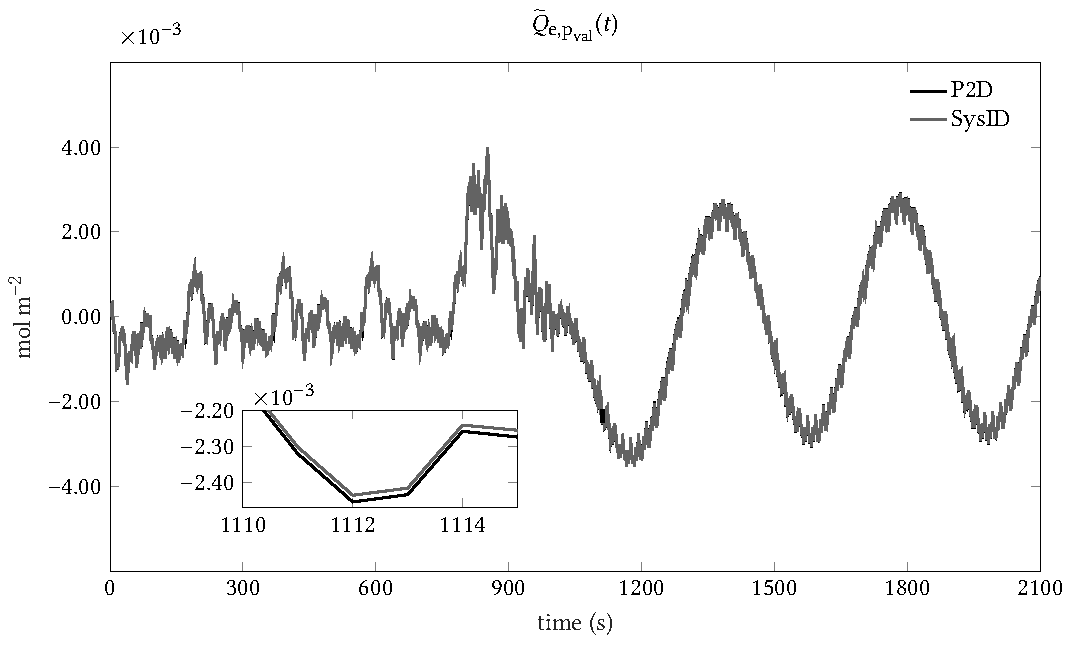
\includegraphics{p2d_sysid_val_qep.pdf}
    \caption[$\widetilde{Q}_{\text{e,p}}(t)$ outputs from \glsfmtshort{p2d} and
    identified transfer function for training profile]{%
        Time-evolution of $\widetilde{Q}_{\text{e,p}}$ computed using the
        \glsfmtshort{p2d} model  and the identified transfer function
        of~\cref{eq:finaldisctfpos} (scaled by 0.001) with the synthetic
        validation input profile of~\cref{fig:sysidvalidationcurrent}. The output
        predicted by the identified transfer function closely matches the `true'
        output obtained by a high-fidelity \glsfmtshort{p2d} simulation with an
        \glsfmtshort{rms} error of \SI{12.07e-6}{\mole\per\meter\squared} and a
        \glsfmtshort{mae} of \SI{31.59e-6}{\mole\per\meter\squared}. Note that the
        transfer function in~\cref{eq:finaldisctfpos} was originally obtained by
        scaling the output by 1000. The transfer function output is
        multiplied by the reciprocal of the same scaling factor to obtain the
        predicted response shown here, thereby once again confirming the
        linearity of this subsystem.
    }%
    \label{fig:tfpredQepval}
\end{figure}

The  poles of~\cref{eq:finaldisctfneg}  lie  very close  to their  corresponding
counterparts of~\cref{eq:finaldisctfpos}  in the  stable region of  the Z-domain
\ie{}  within   the  unit  circle.   This  confirms  the  hypothesis   that  the
time-evolution subsystems  in these  two regions  exhibit similar  dynamics. The
slight differences in  the pole locations could be attributed  to the variations
in  the  physical  parameters  pertaining  to the  two  electrode  regions.  The
numerator coefficients  of~\cref{eq:finaldisctfneg} and~\cref{eq:finaldisctfpos}
are  also  close  to  each  other  except  that  their  signs  are  opposite  to
each   other.  This   is  to   be   expected,  since   as  seen   in  the   step
response   plots   of~\cref{fig:linearity},   $\widetilde{Q}_{\text{e,n}}$   and
$\widetilde{Q}_{\text{e,p}}$ evolve in time in opposite directions. This is also
explained by  the fact  that, for  a given  applied current,  a decrease  in the
number of ions in the negative electrode has to be accompanied by an increase in
the positive electrode and vice-versa (the values of the changes are not exactly
equal owing to the presence of the separator). The identified transfer functions
are thus consistent  and deemed to be suitable for  representing the electrolyte
time-evolution in these regions.

\subsection{Numerical implementation of identified transfer functions}\label{subsec:sysidnumericalimpl}

The  concept of  deploying a  Z-domain  transfer function  may seem  incongruous
to   the  one   of  the   major  goals   of  this   thesis  \viz{}   time-domain
implementation of  \glspl{rom} in an  embedded environment such as  a \gls{bms}.
While  the  majority of  the  models  is  derived  and implemented  entirely  in
time-domain, only  the two  time-evolution subsystems  of the  electrolyte seems
to  deviate  from   this  trajectory.  However,  an  explanation   for  this  is
provided in~\cref{subsec:suitablesysid}.  In particular,  it was  mentioned that
an  approximation-free  conversion to  time-domain  from  Z-domain exists,  that
mitigates this  perceived drawback  for these  two sub-systems.  This conversion
conversion  is  amenable  for  discrete-time implementation  without  any  other
modifications.

Starting from the generic structure of the identified transfer functions (see~\cref{eq:outputwithsysonly}),

\begin{DispWithArrows}[fleqn,mathindent=0cm,jot=2ex,%
    ,xoffset=-4mm
    ]
    G(z) &= \frac{b_1z^{-1} + \dots + b_{n_b}z^{-{n_b}}}{1 + a_1z^{-1} + \dots + a_{n_a}z^{-{n_a}}} \Arrow{Replace with analogous \\ transfer operator $q=z$ \\ in time domain} \notag\\
    G(q) &= \frac{b_1q^{-1} + \dots + b_{n_b}q^{-{n_b}}}{1 + a_1q^{-1} + \dots + a_{n_a}q^{-{n_a}}} \Arrow{Apply the definition\\ of $G(q)$ on the \glsfmtshort{lhs}}\notag \\
    \frac{y[k]}{u[k]} &= \frac{b_1q^{-1} + \dots + b_{n_b}q^{-{n_b}}}{1 + a_1q^{-1} + \dots + a_{n_a}q^{-{n_a}}} \Arrow{Cross-multiply}\notag \\
    \left(1 + a_1q^{-1} + \dots + a_{n_a}q^{-{n_a}}\right)y[k] &= \left(b_1q^{-1} + \dots + b_{n_b}q^{-{n_b}}\right)u[k] \Arrow{Expand on both sides} \notag \\
    y[k] + a_1q^{-1}y[k] + \dots + a_{n_a}q^{-{n_a}}y[k] &= b_1q^{-1}u[k] + \dots + b_{n_b}q^{-{n_b}}u[k] \Arrow{Apply the definition\\ $q^{-p}x[k] = x[k-p]$}\notag \\
    y[k] + a_1y[k-1] + \dots + a_{n_a}y[k-n_a] &= b_1u[k-1] + \dots + b_{n_b}u[k-n_b] \Arrow{Rearrange to obtain\\ the final expression}\notag \\
    y[k] &= -a_1y[k-1] - \dots - a_{n_a}y[k-n_a] \notag \\[-2ex]
         &\qquad   + b_1u[k-1] + \dots + b_{n_b}u[k-n_b] %\label{eq:lccde}
\end{DispWithArrows}

We  thus obtain  a  simple  algebraic expression  (a  difference equation)  that
computes the output  at the given time-step given past  inputs and outputs. This
is a highly memory-efficient implementation  since, at any given time-step, only
the previous $n_a$ (four) output samples  and $n_b$ (four) input samples need to
be  `remembered'  (stored).  This  concludes all  the  aspects  (derivation  and
implementation) of  this author's new  model for the  electrolyte time-evolution
subsystem.  The  performance  of  this  model  for  computation  of  electrolyte
concentration needs to be evaluated, which is performed next.



\section{Performance Analysis of New Model: Ionic Concentration}
% -*- root: ../main.tex -*-
%!TEX root = ../main.tex
% this file is called up by main.tex
% content in this file will be fed into the main document
% vim:textwidth=80 fo=cqt

To demonstrate that a suitable advancement of the field has indeed been achieved
through  this system  identification exercise,  a comparison  with the  existing
state of the art in reduced  order electrolyte modelling is warranted. Secondly,
to  comprehend its  extent of  validity  and performance  boundaries, the  newly
developed \gls{rom} must also be  pitted against the full-order \gls{p2d} model.
This section  aims to  provide such  a comparative discussion  for two  types of
inputs ---
\begin{enumerate*}[label=\itshape\alph*\upshape)]
    \item constant current inputs
    \item dynamic load profiles
\end{enumerate*}

\subsection{Constant current inputs}

\Cref{fig:tfquadp2dspatialionicconc1C} shows  the spatial distribution  of ionic
concentration  in  the electrolyte  along  cell  thickness  for a  1C  discharge
beginning at \SI{100}{\percent} \gls{soc}. The spatial concentration computed by
each of the three approaches ---
\begin{enumerate*}[label=\roman*)]
    \item the \gls{p2d} model,
    \item the quadratic approximation model and
    \item the newly developed system identification model(s).
\end{enumerate*}

\begin{figure}[!htbp]
    \centering
    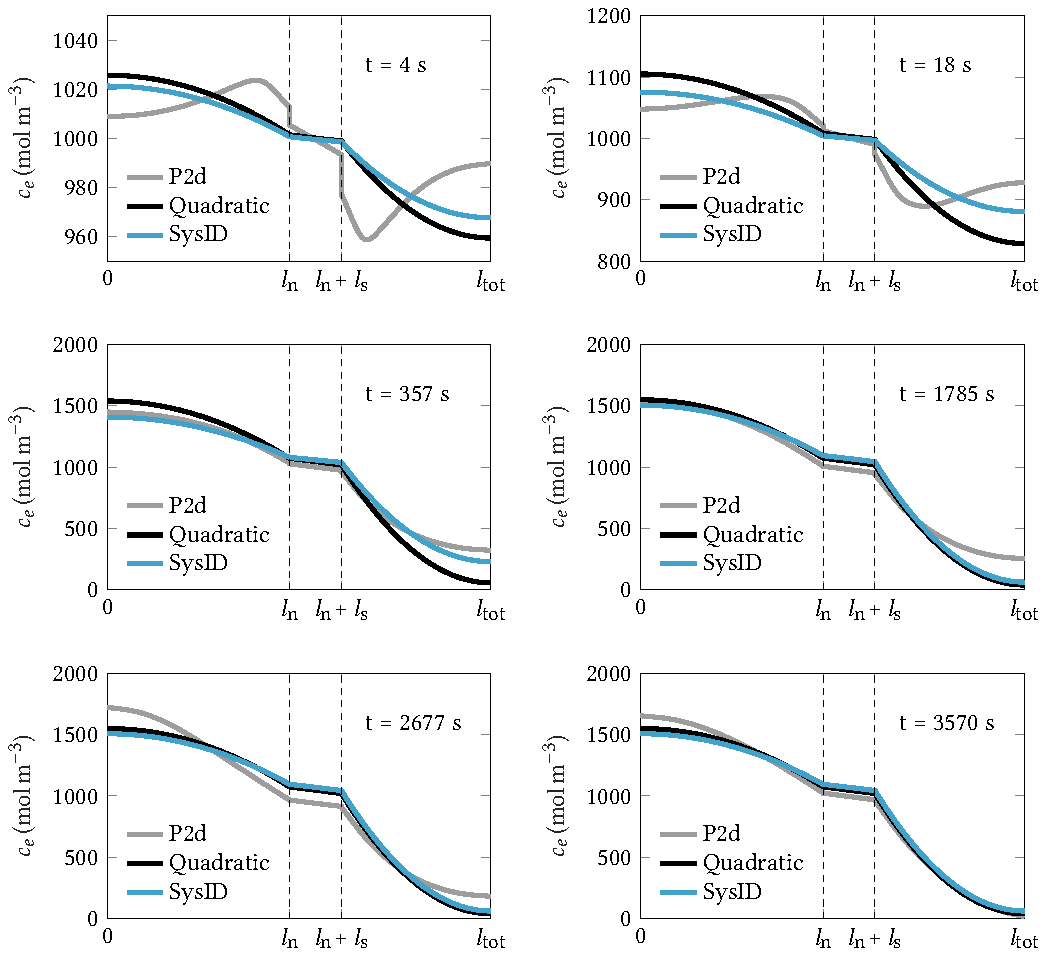
\includegraphics[width=\textwidth]{tf_quadratic_ce_approx_spatial.pdf}
    \caption[Spatial distribution of ionic concentration in
    electrolyte for a 1C discharge computed by the \glsfmtshort{p2d}, quadratic
    approximation \& system identification models]{%
        Spatial distribution of ionic concentration  in electrolyte along cell
        thickness at various  snapshots of  time computed  by each of  the three
        models for  a 1C discharge.  The concentration  profile  computed by
        the  \gls{p2d} model is used as the benchmark reference. The  system
        identification model performs noticeably better than the quadratic
        approximation model during  the initial  transient  while delivering a
        similar performance as a \gls{qss} is reached.
}%
\label{fig:tfquadp2dspatialionicconc1C}
\end{figure}

During  the  initial  phase  of   discharge,  the  \gls{p2d}  model  exhibits  a
characteristic inflection point near the  separator interfaces that diffuses out
over time  until a  \gls{qss}. This  is due to  the fact  the reaction  front is
initially established  close to the  separator, and as surface  concentration of
lithium  in particles  near separator  is  depleted, the  reaction starts  moves
further  into the  electrode thickness.  Neither  of the  two \glspl{rom}  under
consideration here  could successfully  capture this  characteristic inflection.
This is  explained by  the fact  that both  of them  use the  standard quadratic
approximation profile for the \emph{spatial}  profile, which means that only one
apex  point is  possible  per  electrode, which  is  pinned  to their  separator
interfaces by design.

During the transient portion of discharge (approximately up to \SI{357}{\second}
as   shown   in~\cref{fig:tfquadp2dspatialionicconc1C}),   the  locus   of   the
concentration  profile computed  by  the newly  developed system  identification
model(s) clearly lies  much closer to the \gls{p2d} model  than that computed by
the  quadratic  approximation model.  After  the  initial transition  phase,  it
appears  that  the  concentration  profile predicted  by  both  the  \glspl{rom}
converge to the \gls{p2d} model's concentration profile.


To obtain  a quantifiable  perspective on  the accuracy  of the  newly developed
model, it  is desirable  to plot  the temporal  evolution of  the concentration,
particularly  at  the  two  current   collector  interfaces.  The  behaviour  of
the  baseline  quadratic approximation  model  in  this regard  was  established
in~\cref{subsubsec:simresultsbaselinequad}.   Therefore  it   is  important   to
ascertain whether a noteworthy improvement  was achieved using the model arrived
at using the system identification procedure.

\begin{figure}[!htbp]
    \centering
    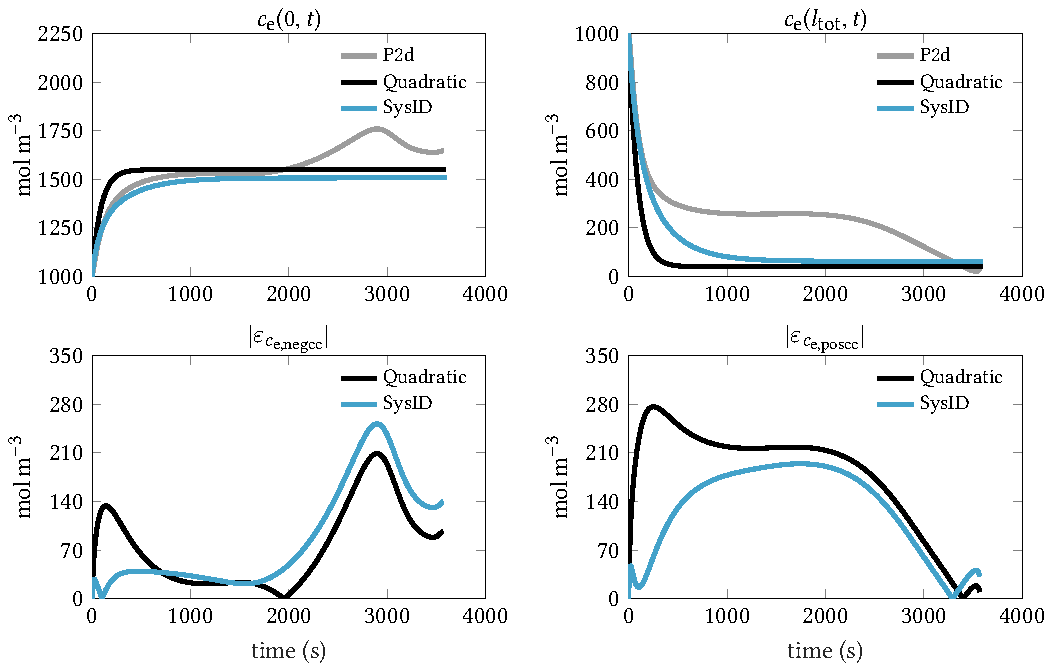
\includegraphics[width=\textwidth]{tf_quad_ce_at_cc_1Cdischg}
    \caption[%
    Time evolution  of ionic  concentrations at  current collectors  computed by
    \glsfmtshort{p2d}, quadratic  approximation \& system  identification models
    for 1C discharge
    ]%
    {%
    Evolution  of ionic  concentration over  time at  the two  current collector
    interfaces for a 1C discharge for
    \begin{enumerate*}[label=\roman*)]
        \item the \glsfmtshort{p2d} model,
        \item the quadratic approximation model and
        \item the newly developed system identification model(s)
    \end{enumerate*}
    (top row). For the quadratic approximation and system identification models,
    the time evolution of their absolute error relative to the \glsfmtshort{p2d}
    benchmark  is also  shown  (bottom  row). At  both  current collectors,  the
    transient performance of the system  identification model is superior to the
    quadratic  approximation model.  At \gls{qss},  the quadratic  approximation
    model is slightly more accurate than the system identification model.
}%
\label{fig:temporalcetfquadratic}
\end{figure}

\Cref{fig:temporalcetfquadratic}   shows  the   time-evolution   of  the   ionic
concentrations at the current collector  interfaces of the negative and positive
electrodes for a 1C discharge. The  concentration profiles computed
by the three approaches ---
\begin{enumerate*}[label=\roman*)]
    \item \glsfmtshort{p2d} model,
    \item quadratic approximation model and the
    \item newly developed system identification model(s)
\end{enumerate*}
are overlaid in the top row of  plots, wherein the left hand side corresponds to
the  current collector  interface  at  the negative  electrode  while the  right
hand  side  corresponds  to  that  at  the  positive  electrode.  The  plots  in
the bottom  row of~\cref{fig:temporalcetfquadratic}  show the  time-evolution of
the  absolute  value  of  their  errors. The  concentration  error  of  each  of
the  two  \glspl{rom}  is  defined  with  respect  to  the  benchmark  \gls{p2d}
model  \ie{}  $\varepsilon_{c_{\text{e,}j}(t)}   =  c_{\text{e,}j_\text{ROM}}  -
c_{\text{e,}j_\text{p2d}}(t)$. The  absolute value  of the  error is  plotted so
that  the magnitude  of the  error can  be visualised  better, aiding  immediate
comparisons based on the plots.

For both  current collectors,  the newly  developed system  identification model
outperforms the  quadratic approximation  model during  the transient  phase. At
the  negative electrode/current  collector interface,  the error  of the  system
identification model remains strictly below  that of the quadratic approximation
model until \approx \SI{650}{\second} and remains comparable to it until \approx
\SI{1600}{\second}. Beyond  this time, the  quadratic approximation model  has a
slightly better accuracy, although the system identification model still remains
at a comparable distance from  it. After \approx \SI{2000}{\second}, both models
yield  the same  response shape.  For the  positive electrode/current  collector
interface, the  error of the system  identification model remains below  that of
the quadratic approximation model until \approx \SI{3300}{\second}.

\begin{figure}[!htbp]
    \centering
    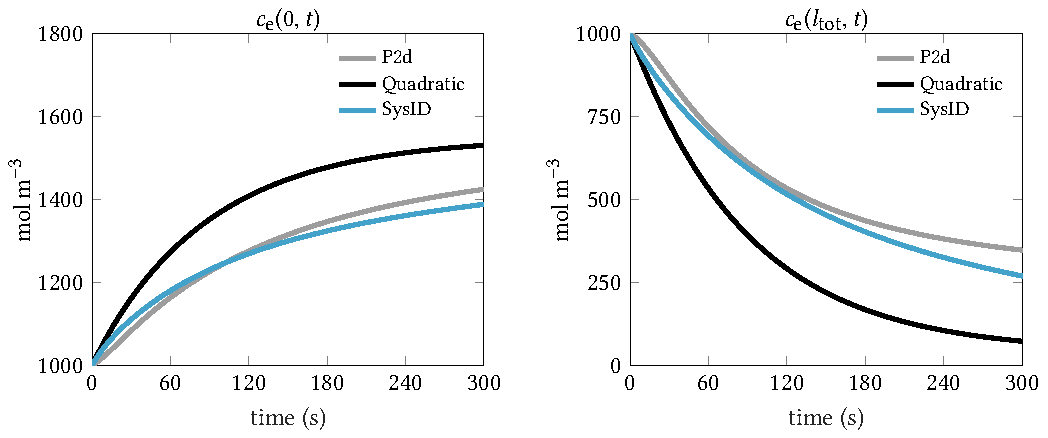
\includegraphics[width=\textwidth]{zoomed_tf_quad_ce_at_cc_1Cdischg.pdf}
    \caption[%
    Transient phase of ionic  concentration evolution at  the two current collectors  computed by
    \glsfmtshort{p2d}, quadratic  \& system  identification models
    for 1C discharge
    ]%
    {%
    Transient phase of the temporal evolution  of ionic  concentration at  the two  current collector
    interfaces for a 1C discharge as computed by ---
    \begin{enumerate*}[label=\roman*)]
        \item the \glsfmtshort{p2d} model,
        \item the quadratic approximation model, and
        \item the newly developed system identification model(s).
    \end{enumerate*}
    The significantly improved accuracy of the system identification model(s)
    relative to the state of the art quadratic approximation model is clearly demonstrated.
}%
\label{fig:zoomedcetfquadtemporal}
\end{figure}

\Cref{fig:zoomedcetfquadtemporal} shows  a zoomed version of  the time-evolution
of the  ionic concentration  at the  two current  collectors, wherein  the first
\SI{300}{\second}  after  application  of  the  load  current  is  plotted.  The
significant  improvement in  accuracy  achieved by  the  newly developed  system
identification model(s) is clearly demonstrated. At both the current collectors,
the concentration computed  by the system identification  model(s) closely track
that of the benchmark \gls{p2d} model.

The  loss  of fidelity  exhibited  past  the  initial transient  phase  warrants
an  explanation. It  should  be  recalled that  the  natural  decoupling of  the
temporal and  spatial systems were taken  advantage of in developing  the system
identification technique. This  means that, for the spatial  profile, the system
identification  model reverts  to the  same  quadratic profile  as the  baseline
quadratic approximation  model. This  explains why the  two models  have similar
shape past the initial transient. During  the transient phase when the \gls{qss}
behaviour is yet to be established, it is reasonable to assume that the temporal
dynamics  are of  paramount importance  in governing  the concentration  profile
evolution.  After a  \gls{qss}  has  been established  with  the reaction  front
diffusing out  and a steady  stream of ion-electron  separation/recombination in
place,  it is  hypothesised  that the  temporal dynamics  have  settled and  the
spatial configuration assumes importance.

With a  sustained application  of constant current  past the  initial transient,
strong spatial gradients  in the ionic concentration are  established within the
cell \ie{} the  concentrations are far from the initial  equilibrium value. This
precisely  exposes the  realm  where the  system  identification model  exhibits
its  natural  weakness.  By  following  the  theory  of  system  identification,
which  necessitates   bias  removal,   the  training  and   validation  profiles
of~\cref{fig:sysidtrainingcurrent}   and~\cref{fig:sysidvalidationcurrent}   had
nearly  zero mean.  This means  that the  currents were  as equally  positive as
negative leading to a small-signal  perturbation around the equilibrium value of
the electrolyte  concentration. While this  profile is ideally suited  to excite
the system's  dynamics, it  fails to  capture the large  signal behaviour.  As a
topic  of future  research,  perhaps a  spatially-coupled system  identification
could be attempted to handle this issue.

The  main  implication of  these  results  is  that  the identified  models  are
primarily suitable for  transient \ie{} dynamic load profiles,  which is typical
of a real-life scenario in an electric/hybrid electric vehicular operation. Such
a  model is  less  suitable  for sustained  constant  current application.  This
implies that  a \gls{bms} in a  vehicle undergoing a \gls{cccv}  charging cannot
rely on  these identified electrolyte  models. However, this exclusion  does not
seriously hamper the model's wider applicability since a simple coulomb-counting
approach with  a high-precision \gls{adc} is  much more accurate than  any other
physics based model in this particular scenario.

Although constant  current discharge is  not a practical use-case  for vehicular
batteries, performing this benchmark evaluation  has helped in understanding the
limits of the newly  developed model. This study has also  helped in providing a
glimpse of its  potential strength \viz{} significantly  improved accuracy under
dynamic load conditions, which is presented next.

\subsection{Dynamic load profiles}


\begin{figure}[!htbp]
    \centering
    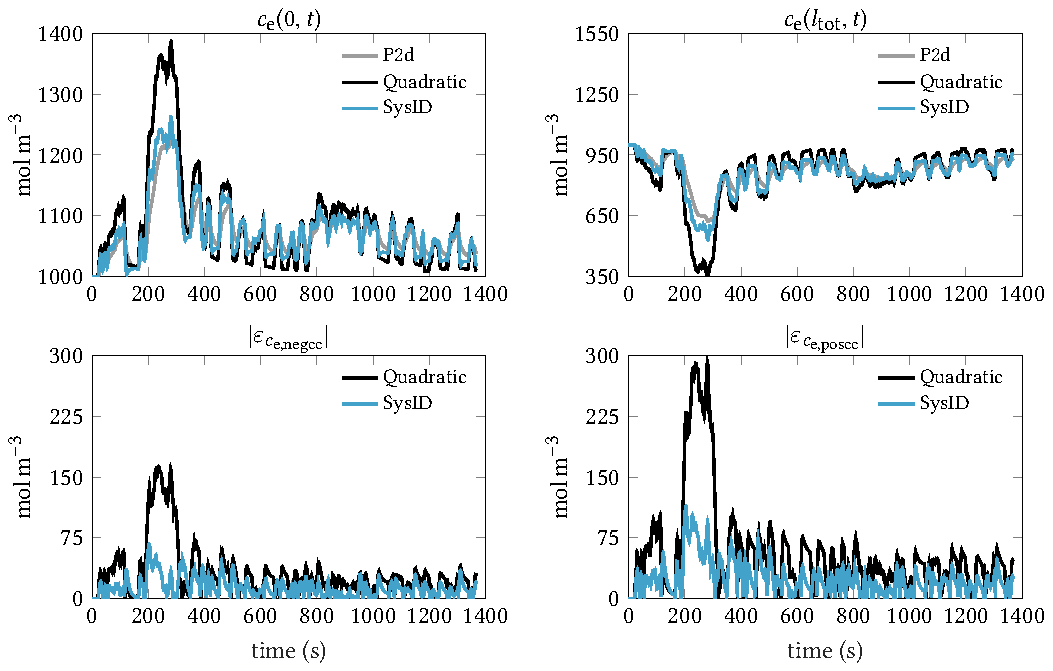
\includegraphics[width=\textwidth]{tf_quad_ce_at_cc_udds}
    \caption{}
    \label{}
\end{figure}

\begin{figure}[!htbp]
    \centering
    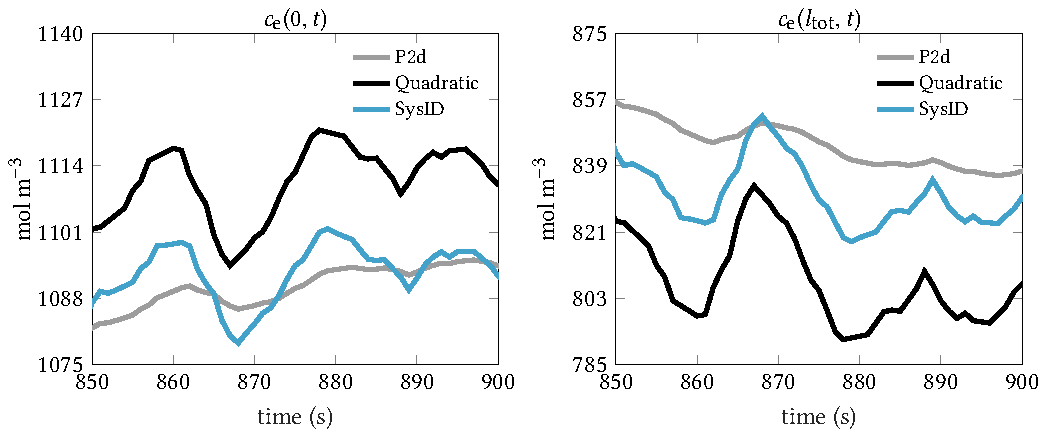
\includegraphics[width=\textwidth]{zoomed_tf_quad_ce_at_cc_udds}
    \caption{}
    \label{}
\end{figure}



% \section{Embedding into SPM and final results for composite system}

% % Assumed transfer function model. Test results within the model itself
% % Test results for electrolyte ce (subsection)
% % test results for full system (final section)

% % mention in introduction where code snippets are given



